% Options for packages loaded elsewhere
\PassOptionsToPackage{unicode}{hyperref}
\PassOptionsToPackage{hyphens}{url}
\documentclass[
]{article}
\usepackage{xcolor}
\usepackage{amsmath,amssymb}
\setcounter{secnumdepth}{5}
\usepackage{iftex}
\ifPDFTeX
  \usepackage[T1]{fontenc}
  \usepackage[utf8]{inputenc}
  \usepackage{textcomp} % provide euro and other symbols
\else % if luatex or xetex
  \usepackage{unicode-math} % this also loads fontspec
  \defaultfontfeatures{Scale=MatchLowercase}
  \defaultfontfeatures[\rmfamily]{Ligatures=TeX,Scale=1}
\fi
% \usepackage{lmodern}
\ifPDFTeX\else
  % xetex/luatex font selection
\fi
% Use upquote if available, for straight quotes in verbatim environments
\IfFileExists{upquote.sty}{\usepackage{upquote}}{}
\IfFileExists{microtype.sty}{% use microtype if available
  \usepackage[]{microtype}
  \UseMicrotypeSet[protrusion]{basicmath} % disable protrusion for tt fonts
}{}
\makeatletter
\@ifundefined{KOMAClassName}{% if non-KOMA class
  \IfFileExists{parskip.sty}{%
    \usepackage{parskip}
  }{% else
    \setlength{\parindent}{0pt}
    \setlength{\parskip}{6pt plus 2pt minus 1pt}}
}{% if KOMA class
  \KOMAoptions{parskip=half}}
\makeatother
\usepackage{color}
\usepackage{fancyvrb}
\newcommand{\VerbBar}{|}
\newcommand{\VERB}{\Verb[commandchars=\\\{\}]}
\DefineVerbatimEnvironment{Highlighting}{Verbatim}{commandchars=\\\{\}}
% Add ',fontsize=\small' for more characters per line
\newenvironment{Shaded}{}{}
\newcommand{\AlertTok}[1]{\textcolor[rgb]{1.00,0.00,0.00}{\textbf{#1}}}
\newcommand{\AnnotationTok}[1]{\textcolor[rgb]{0.38,0.63,0.69}{\textbf{\textit{#1}}}}
\newcommand{\AttributeTok}[1]{\textcolor[rgb]{0.49,0.56,0.16}{#1}}
\newcommand{\BaseNTok}[1]{\textcolor[rgb]{0.25,0.63,0.44}{#1}}
\newcommand{\BuiltInTok}[1]{\textcolor[rgb]{0.00,0.50,0.00}{#1}}
\newcommand{\CharTok}[1]{\textcolor[rgb]{0.25,0.44,0.63}{#1}}
\newcommand{\CommentTok}[1]{\textcolor[rgb]{0.38,0.63,0.69}{\textit{#1}}}
\newcommand{\CommentVarTok}[1]{\textcolor[rgb]{0.38,0.63,0.69}{\textbf{\textit{#1}}}}
\newcommand{\ConstantTok}[1]{\textcolor[rgb]{0.53,0.00,0.00}{#1}}
\newcommand{\ControlFlowTok}[1]{\textcolor[rgb]{0.00,0.44,0.13}{\textbf{#1}}}
\newcommand{\DataTypeTok}[1]{\textcolor[rgb]{0.56,0.13,0.00}{#1}}
\newcommand{\DecValTok}[1]{\textcolor[rgb]{0.25,0.63,0.44}{#1}}
\newcommand{\DocumentationTok}[1]{\textcolor[rgb]{0.73,0.13,0.13}{\textit{#1}}}
\newcommand{\ErrorTok}[1]{\textcolor[rgb]{1.00,0.00,0.00}{\textbf{#1}}}
\newcommand{\ExtensionTok}[1]{#1}
\newcommand{\FloatTok}[1]{\textcolor[rgb]{0.25,0.63,0.44}{#1}}
\newcommand{\FunctionTok}[1]{\textcolor[rgb]{0.02,0.16,0.49}{#1}}
\newcommand{\ImportTok}[1]{\textcolor[rgb]{0.00,0.50,0.00}{\textbf{#1}}}
\newcommand{\InformationTok}[1]{\textcolor[rgb]{0.38,0.63,0.69}{\textbf{\textit{#1}}}}
\newcommand{\KeywordTok}[1]{\textcolor[rgb]{0.00,0.44,0.13}{\textbf{#1}}}
\newcommand{\NormalTok}[1]{#1}
\newcommand{\OperatorTok}[1]{\textcolor[rgb]{0.40,0.40,0.40}{#1}}
\newcommand{\OtherTok}[1]{\textcolor[rgb]{0.00,0.44,0.13}{#1}}
\newcommand{\PreprocessorTok}[1]{\textcolor[rgb]{0.74,0.48,0.00}{#1}}
\newcommand{\RegionMarkerTok}[1]{#1}
\newcommand{\SpecialCharTok}[1]{\textcolor[rgb]{0.25,0.44,0.63}{#1}}
\newcommand{\SpecialStringTok}[1]{\textcolor[rgb]{0.73,0.40,0.53}{#1}}
\newcommand{\StringTok}[1]{\textcolor[rgb]{0.25,0.44,0.63}{#1}}
\newcommand{\VariableTok}[1]{\textcolor[rgb]{0.10,0.09,0.49}{#1}}
\newcommand{\VerbatimStringTok}[1]{\textcolor[rgb]{0.25,0.44,0.63}{#1}}
\newcommand{\WarningTok}[1]{\textcolor[rgb]{0.38,0.63,0.69}{\textbf{\textit{#1}}}}
\usepackage{longtable,booktabs,array}
\newcounter{none} % for unnumbered tables
\usepackage{calc} % for calculating minipage widths
% Correct order of tables after \paragraph or \subparagraph
\usepackage{etoolbox}
\makeatletter
\patchcmd\longtable{\par}{\if@noskipsec\mbox{}\fi\par}{}{}
\makeatother
% Allow footnotes in longtable head/foot
\IfFileExists{footnotehyper.sty}{\usepackage{footnotehyper}}{\usepackage{footnote}}
\makesavenoteenv{longtable}
\usepackage{graphicx}
\makeatletter
\newsavebox\pandoc@box
\newcommand*\pandocbounded[1]{% scales image to fit in text height/width
  \sbox\pandoc@box{#1}%
  \Gscale@div\@tempa{\textheight}{\dimexpr\ht\pandoc@box+\dp\pandoc@box\relax}%
  \Gscale@div\@tempb{\linewidth}{\wd\pandoc@box}%
  \ifdim\@tempb\p@<\@tempa\p@\let\@tempa\@tempb\fi% select the smaller of both
  \ifdim\@tempa\p@<\p@\scalebox{\@tempa}{\usebox\pandoc@box}%
  \else\usebox{\pandoc@box}%
  \fi%
}
% Set default figure placement to htbp
\def\fps@figure{htbp}
\makeatother
\setlength{\emergencystretch}{3em} % prevent overfull lines
\providecommand{\tightlist}{%
  \setlength{\itemsep}{0pt}\setlength{\parskip}{0pt}}
\usepackage[]{natbib}
\bibliographystyle{plainnat}
\usepackage{bookmark}
\IfFileExists{xurl.sty}{\usepackage{xurl}}{} % add URL line breaks if available
\urlstyle{same}
\hypersetup{
  colorlinks=true,linkcolor=red,urlcolor=red,citecolor=red,anchorcolor=red,
  pdfcreator={LaTeX via pandoc}}

\author{}
\date{}

\title{Convergence Analysis of Gradient Descent Optimization\\\normalsize Theoretical Bounds and Empirical Performance in Quadratic Minimization}
\author{Research Template Author\\\footnotesize{Research Template Institute}\\\footnotesize{\texttt{author@research-template.org}}\\\footnotesize{\href{https://orcid.org/0000-0000-0000-1234}{ORCID: 0000-0000-0000-1234}} \\and Co-Author\\\footnotesize{Department of Computational Mathematics}\\\footnotesize{\texttt{coauthor@research-template.org}}\\\footnotesize{\href{https://orcid.org/0000-0000-0000-5678}{ORCID: 0000-0000-0000-5678}} \\ \footnotesize{\href{https://doi.org/10.5281/zenodo.12345678}{DOI: 10.5281/zenodo.12345678}}}
\date{\today}

% Core mathematics
\usepackage{amsmath}
\usepackage{amssymb}
\usepackage{amsfonts}
\usepackage{amsthm}

% Document layout
\usepackage{geometry}
\usepackage{float}
\usepackage{graphicx}

% Tables
\usepackage{booktabs}
\usepackage{longtable}
\usepackage{array}

% Algorithm typesetting (for pseudocode in §2 Methodology)
\usepackage[ruled,vlined,linesnumbered]{algorithm2e}

% Code listings
\usepackage{listings}

% Typography and formatting
\usepackage{microtype}
\usepackage{xcolor}
\usepackage[binary-units]{siunitx}

% Cross-references and citations
\usepackage{hyperref}
\hypersetup{
    colorlinks=true,
    allcolors=red
}
\usepackage[capitalise,noabbrev]{cleveref}
\usepackage{natbib}

\begin{document}

\maketitle
\thispagestyle{empty}
\tableofcontents
\newpage


\section{Abstract}\label{abstract}

This paper presents a convergence study of \textbf{fixed-step gradient
descent} on a convex quadratic, framed as the computational exemplar of
the \href{https://github.com/docxology/template}{Research Project
Template}. The implementation lives in
\texttt{projects/code\_project/src/optimizer.py}; experiments and
figures are orchestrated by
\texttt{projects/code\_project/scripts/optimization\_analysis.py} and
hydrated into the manuscript through
\texttt{scripts/z\_generate\_manuscript\_variables.py}, so tables and
prose track \texttt{output/data/optimization\_results.csv} after every
pipeline run.

We evaluate 6 step sizes from \(\alpha = 0.01\) to \(\alpha = 2.5\),
spanning conservative, near-optimal, aggressive, and divergent regimes
for a unit Hessian model. The build chain exercises template
infrastructure end-to-end: scientific helpers
(\texttt{infrastructure.scientific.stability},
\texttt{infrastructure.scientific.benchmarking}), validation, rendering
(\texttt{infrastructure/rendering/pdf\_renderer.py}), and reporting.
Accessibility-oriented plotting defaults (colourblind-safe palette,
300\,dpi exports) are centralized in \texttt{optimization\_analysis.py}.

Contributions are \textbf{methodological} and \textbf{architectural}. On
the methods side, we relate empirical iteration counts and error decay
to the scalar contraction factor \(\rho(\alpha) = |1-\alpha|\) and
document cases where runs hit \(N_{\max} = 1000\) before meeting the
gradient tolerance. On the architecture side, we demonstrate a zero-mock
test suite on project \texttt{src/} (see
\href{https://github.com/docxology/template/blob/main/projects/code_project/tests/test_optimizer.py}{test\_optimizer.py}),
automated six-figure analysis, and reproducibility metadata
(configuration hash, artifact counts) injected into Section 6.

\textbf{Results (this configuration):} 4 of 6 grid points report
\texttt{converged=True} in the CSV; non-convergent rows flag either slow
progress at small \(\alpha) under the iteration cap or instability when
\(|1-\alpha| \geq 1\). The analytical minimizer remains \(x^\ast = 1.0\)
with \(f(x^\ast) = -0.5\) for the configured \((A,b)\).

\textbf{Keywords:} gradient descent, reproducible research, zero-mock
testing, scientific infrastructure, pipeline orchestration

\newpage

\section{Introduction}\label{introduction}

This \texttt{code\_project} serves as the foundational exemplar for the
\href{https://github.com/docxology/template}{Research Project Template}
ecosystem, demonstrating a fully-tested numerical optimization
implementation securely bracketed by rigorous infrastructure, hermetic
testing, and extensive documentation architectures. The words you are
reading---and the mathematical figures below them---have been
programmably generated through an unbreakable custody chain starting
from algorithm implementation through strict CI/CD validation to
multi-format \texttt{.pdf} compilation.

\subsection{Template Architecture
Context}\label{template-architecture-context}

Scientific engineering requires mathematical accuracy combined with
software reliability. This project unifies theoretical optimization with
the repository's three foundational pillars:

\begin{enumerate}
\def\labelenumi{\arabic{enumi}.}
\tightlist
\item
  \textbf{\texttt{infrastructure/} Layer (Root Directory)}: A modular
  stack of nine subpackages (\texttt{core}, \texttt{validation},
  \texttt{scientific}, \texttt{rendering}, \texttt{reporting},
  \texttt{documentation}, \texttt{llm}, \texttt{publishing},
  \texttt{project}) providing the computational scaffolding.
\item
  \textbf{\texttt{tests/} Framework
  (\texttt{projects/code\_project/tests/})}: An uncompromising
  validation layer maintaining a zero-mock testing policy. This is
  enforced automatically via the
  \href{https://github.com/docxology/template/blob/main/.github/workflows/ci.yml}{CI
  workflow} mapping to \texttt{pyproject.toml} directives.
\item
  \textbf{\texttt{docs/} Knowledge Base
  (\texttt{projects/code\_project/docs/})}: A structured repository of
  architectural guidelines, operational patterns, and the Rigorous
  Agentic Scientific Protocol (RASP) that governs the AI-assisted agents
  writing these very texts.
\end{enumerate}

This implementation of gradient descent algorithms for solving
optimization problems is used as the vehicle to demonstrate these
pillars. The theoretical problem is mapped programmatically inside the
\href{https://github.com/docxology/template/blob/main/projects/code_project/src/optimizer.py}{optimizer
module}:

\begin{equation}
\label{eq:optimization_problem}
\min_{x \in \mathbb{R}^n} f(x)
\end{equation}

where \(f: \mathbb{R}^n \rightarrow \mathbb{R}\) is a continuously
differentiable objective function.

\subsection{Infrastructure
Integration}\label{infrastructure-integration}

Rather than existing as isolated scripts, this project extensively
leverages the \texttt{infrastructure} layer:

\begin{itemize}
\tightlist
\item
  \textbf{Scientific Utilities}: Utilizing
  \texttt{infrastructure.scientific.stability} and
  \texttt{infrastructure.scientific.benchmarking} to guarantee numerical
  boundaries and performance scaling.
\item
  \textbf{Hermetic Validation}: Deploying
  \texttt{infrastructure.validation} components
  (\texttt{markdown\_validator}, \texttt{output\_validator}) to ensure
  all generated artifacts are cryptographically sound.
\item
  \textbf{Reporting \& Rendering}: Employing
  \texttt{infrastructure.rendering.pdf\_renderer} and
  \texttt{infrastructure.reporting.executive\_reporter} to automatically
  transform code outputs into this finalized manuscript.
\end{itemize}

\subsection{Algorithm Overview}\label{algorithm-overview}

The reference gradient descent algorithm iteratively updates the
solution using:

\begin{equation}
\label{eq:gradient_descent_update}
x_{k+1} = x_k - \alpha \nabla f(x_k)
\end{equation}

where \(\alpha > 0\) is the step size (learning rate) and
\(\nabla f(x_k)\) is the gradient of the objective function at iteration
\(k\).

\subsection{Exemplar Implementation
Goals}\label{exemplar-implementation-goals}

As the representative project for the repository, this implementation
explicitly demonstrates:

\begin{enumerate}
\def\labelenumi{\arabic{enumi}.}
\tightlist
\item
  \textbf{Infrastructure-Coupled Code}: Scientific implementations that
  delegate logging, file ops, and reporting to the
  \texttt{infrastructure} core.
\item
  \textbf{Zero-Mock Verification}: A strict comprehensive validation
  suite proving numerical accuracy without artificial test boundaries.
\item
  \textbf{Automated Research Pipelines}: High-precision analyses that
  generate publication-quality, accessible visualizations automatically.
\item
  \textbf{Agentic Documentation standards}: Native adherence to the RASP
  methodology and \texttt{AGENTS.md} guidelines, ensuring the logic
  remains verifiable by both human and artificial intelligence.
\end{enumerate}

\subsection{Reader's guide to the
manuscript}\label{readers-guide-to-the-manuscript}

\begin{itemize}
\tightlist
\item
  \textbf{Section 2 (Methodology)} ties pseudocode to
  \texttt{gradient\_descent()} and explains how stability checks and
  benchmarks call into \texttt{infrastructure.scientific}.
\item
  \textbf{Section 3 (Results)} is figure-centric: every panel references
  the generator function in \texttt{optimization\_analysis.py} and uses
  \texttt{\{\{CONFIG\_*\}\}} / \texttt{\{\{RESULT\_*\}\}} placeholders
  for numeric values.
\item
  \textbf{Section 5 (Experimental setup)} lists the exact YAML fields
  (\texttt{experiment:} block) that controlled the run whose artifacts
  you are viewing.
\item
  \textbf{Section 6 (Reproducibility)} records the configuration hash
  and artifact inventory produced alongside the PDF.
\item
  \textbf{Section 7} states scope and related literature so the exemplar
  is not mistaken for a general-purpose optimizer benchmark suite.
\end{itemize}

\subsection{Why a quadratic model}\label{why-a-quadratic-model}

Restricting \(f\) to a quadratic with known \((A,b)\) keeps the optimum,
gradient, and spectral data explicit. For \(A = I\) and
\(b = \mathbf{1}\), the optimal point is \(x^\ast = \mathbf{1}\) and
gradient descent with fixed \(\alpha) reduces to a linear iteration in
the error (see Equation \ref{eq:scalar_linear_update} in the results
section). That simplicity isolates step-size effects and makes divergent
choices (\(\alpha \geq 2\) in 1D) visible in both plots and CSV rows
without requiring trust-region or line-search fixes---those extensions
are left to future work (Section 7).

\newpage

\section{Methodology}\label{methodology}

This section describes the implementation methodology, explicitly
detailing how the optimization algorithms are constructed, validated,
and analyzed using the Generalized Research Template's
\texttt{infrastructure} and \texttt{tests} ecosystems.

\subsection{Algorithm Implementation}\label{algorithm-implementation}

\subsubsection{Gradient Descent
Algorithm}\label{gradient-descent-algorithm}

The core algorithm implements the iterative procedure for unconstrained
optimization. Crucially, the implementation is designed to be highly
observable, delegating all logging to
\texttt{infrastructure.core.logging.utils.ProjectLogger} and executing
under the hermetic boundaries defined in the
\href{https://github.com/docxology/template/blob/main/projects/code_project/tests/conftest.py}{test
configuration}.

\textbf{Algorithm 1: Gradient Descent (implemented in the
\href{https://github.com/docxology/template/blob/main/projects/code_project/src/optimizer.py\#L42-L138}{optimizer
module})}

\begin{quote}
\textbf{Input:} Initial point \(x_0\), step size \(\alpha), tolerance
\(\epsilon\), max iterations \(N_{\max}\)

\begin{enumerate}
\def\labelenumi{\arabic{enumi}.}
\tightlist
\item
  Initialize \(k \leftarrow 0\)
\item
  \textbf{While} \(k < N_{\max}\) \textbf{do:}

  \begin{itemize}
  \tightlist
  \item
    Compute gradient \(g_k = \nabla f(x_k)\)
  \item
    \textbf{If} \(\|g_k\|_2 < \epsilon\) \textbf{then return} \(x_k\)
    \emph{(converged)}
  \item
    Update: \(x_{k+1} \leftarrow x_k - \alpha \cdot g_k\)
  \item
    \(k \leftarrow k + 1\)
  \end{itemize}
\item
  \textbf{Return} \(x_k\) \emph{(max iterations reached)}
\end{enumerate}
\end{quote}

\subsection{Infrastructure
Integration}\label{infrastructure-integration-1}

The methodology explicitly bridges theoretical mathematics with
production-grade validation through the
\texttt{infrastructure.scientific} module.

\subsubsection{Numerical Stability
Analysis}\label{numerical-stability-analysis}

Rather than writing ad-hoc validation code, the project imports
\texttt{infrastructure.scientific.stability.check\_numerical\_stability}.
This utility subjects the objective function to a barrage of extreme
inputs (NaN, Inf, \(\pm 10^{10}\)) to calculate a formalized stability
score. If this score degrades, the
\href{https://github.com/docxology/template/blob/main/scripts/02_run_analysis.py}{analysis
orchestrator} execution deliberately aborts, ensuring the methodology
cannot enter unrecoverable states.

\subsubsection{Performance Benchmarking}\label{performance-benchmarking}

Computational complexity is evaluated not just theoretically, but
empirically via
\href{https://github.com/docxology/template/blob/main/infrastructure/scientific/benchmarking.py}{\texttt{infrastructure.scientific.benchmarking.benchmark\_function}}.
This module captures high-resolution execution timings and memory
footprints across dimensionality sweeps, guaranteeing that the \(O(n)\)
space-time complexity predictions hold true on the host architecture.

\subsection{Convergence Analysis}\label{convergence-analysis}

For quadratic functions \(f(x) = \frac{1}{2}x^T A x - b^T x\) where
\(A\) is positive definite, the convergence factor becomes
\cite{bertsekas1999nonlinear}:

\begin{equation}
\label{eq:convergence_factor}
\rho = \frac{|\lambda_{\max} - \alpha\lambda_{\min}|}{|\lambda_{\min} + \alpha\lambda_{\max}|}
\end{equation}

Optimal convergence occurs when
\(\alpha = \frac{2}{\lambda_{\min} + \lambda_{\max}}\), yielding
\(\rho = \frac{\kappa - 1}{\kappa + 1}\).

\subsection{Experimental Setup}\label{experimental-setup}

\subsubsection{Step Size Analysis}\label{step-size-analysis}

Step sizes are not chosen ad hoc in the manuscript: they are read from
\texttt{experiment.step\_sizes} in \texttt{manuscript/config.yaml} and
passed through \texttt{run\_convergence\_experiment()} in
\texttt{optimization\_analysis.py}. The active grid for this build is:

\begin{itemize}
\tightlist
\item
  \(\\alpha = 0.01\) (conservative)
\item
  \(\\alpha = 0.1\) (conservative)
\item
  \(\\alpha = 0.5\) (near-optimal)
\item
  \(\\alpha = 1.0\) (near-optimal)
\item
  \(\\alpha = 1.5\) (aggressive)
\item
  \(\\alpha = 2.5\) (divergent (expected unstable for H = I))
\end{itemize}

Labels follow the same agency taxonomy used for plot colours
(\texttt{\_agency\_category} in the analysis script):
\textbf{conservative} (small \(\alpha), slow but stable on \(H=I\)),
\textbf{near-optimal} (including \(\alpha=1\) where the method reaches
\(x^\ast\) in one step for this quadratic), \textbf{aggressive}
(\(1 < \alpha < 2\), still linearly contracting in \(|x-x^\ast|\) but
oscillatory in sign), and \textbf{divergent} (\(|1-\alpha| \geq 1\)).

\subsubsection{Zero-Mock Testing
Methodology}\label{zero-mock-testing-methodology}

The most critical aspect of the project's methodology is its validation
framework. The project is governed by a strict Zero-Mock testing policy,
evaluated actively by executing
\texttt{uv\ run\ pytest\ projects/code\_project/tests/} during the
infrastructure build phase.

\begin{enumerate}
\def\labelenumi{\arabic{enumi}.}
\tightlist
\item
  \textbf{Integration Testing}: The \texttt{tests/integration/} battery
  ensures that the optimization algorithm, the analysis pipeline, and
  the \texttt{infrastructure.rendering} components operate flawlessly
  together without simulated data.
\item
  \textbf{Infrastructure Validation}: The \texttt{tests/infra\_tests/}
  suite confirms that the underlying modules (e.g.,
  \texttt{pipeline\_reporter.py}, \texttt{doc\_discovery.py}) behave
  deterministically.
\item
  \textbf{Coverage Gates}: The
  \href{https://github.com/docxology/template/blob/main/.github/workflows/ci.yml}{GitHub
  Actions CI workflow} enforces a mandatory ≥90\% statement coverage
  gate on \texttt{projects/code\_project/src/} prior to treating the
  project as build-green.
\end{enumerate}

\subsubsection{Stopping rule and
reporting}\label{stopping-rule-and-reporting}

\texttt{gradient\_descent()} terminates when \(\|\nabla f(x_k)\|\) falls
below \texttt{experiment.tolerance} or when \(k\) reaches
\texttt{experiment.max\_iterations}. The boolean \texttt{converged} in
exported CSV rows distinguishes these outcomes. Downstream,
\texttt{scripts/z\_generate\_manuscript\_variables.py} aggregates the
CSV into \texttt{RESULT\_*} placeholders so tables and prose cannot
drift from the last analysis run.

\subsubsection{Figure generation
contract}\label{figure-generation-contract}

Each figure in \texttt{03\_results.md} maps to a single generator in
\texttt{optimization\_analysis.py}
(\texttt{generate\_convergence\_plot},
\texttt{generate\_step\_size\_sensitivity\_plot},
\texttt{generate\_convergence\_rate\_plot},
\texttt{generate\_complexity\_visualization},
\texttt{generate\_stability\_visualization},
\texttt{generate\_benchmark\_visualization}). Captions in the markdown
intentionally name the function and the key parameters (tolerance lines,
grids, dimensions) so reviewers can navigate from PDF to code without
inferring hidden defaults.

\subsection{Analysis Pipeline \& LaTeX
Integration}\label{analysis-pipeline-latex-integration}

The automated analysis script leverages
\texttt{infrastructure.core.progress.PipelineProgress} to orchestrate
experiments, collect convergence trajectories, and generate
publication-quality visualizations seamlessly.

The research template supports advanced LaTeX customization through the
\texttt{preamble.md} configuration. This is ingested directly by
\texttt{infrastructure.rendering.latex\_utils.py} and
\texttt{pdf\_renderer.py}, automatically linking compiled PGF plots and
BibTeX citations. This automated approach ensures an unbreakable chain
of custody from raw algorithmic execution to the final rendered
manuscript.

\newpage

\section{Results}\label{results}

This section presents the experimental results from the gradient descent
optimization study, including convergence analysis and performance
comparisons. Every table, figure, and quantitative assertion in this
section was compiled autonomously by the template's
\texttt{infrastructure.reporting} subsystem executing the
\href{https://github.com/docxology/template/blob/main/projects/code_project/scripts/optimization_analysis.py}{optimization
analysis script}. No manual transcription was permitted.

\subsection{Convergence Analysis}\label{convergence-analysis-1}

\subsubsection{Convergence Trajectories}\label{convergence-trajectories}

Figure \ref{fig:convergence} illustrates the convergence behavior of
gradient descent for different step sizes, starting from the initial
point \(x_0 = 0\). The algorithm iteratively updates the solution using
the rule \(x_{k+1} = x_k - \alpha \nabla f(x_k)\).

\begin{figure}
\centering
\pandocbounded{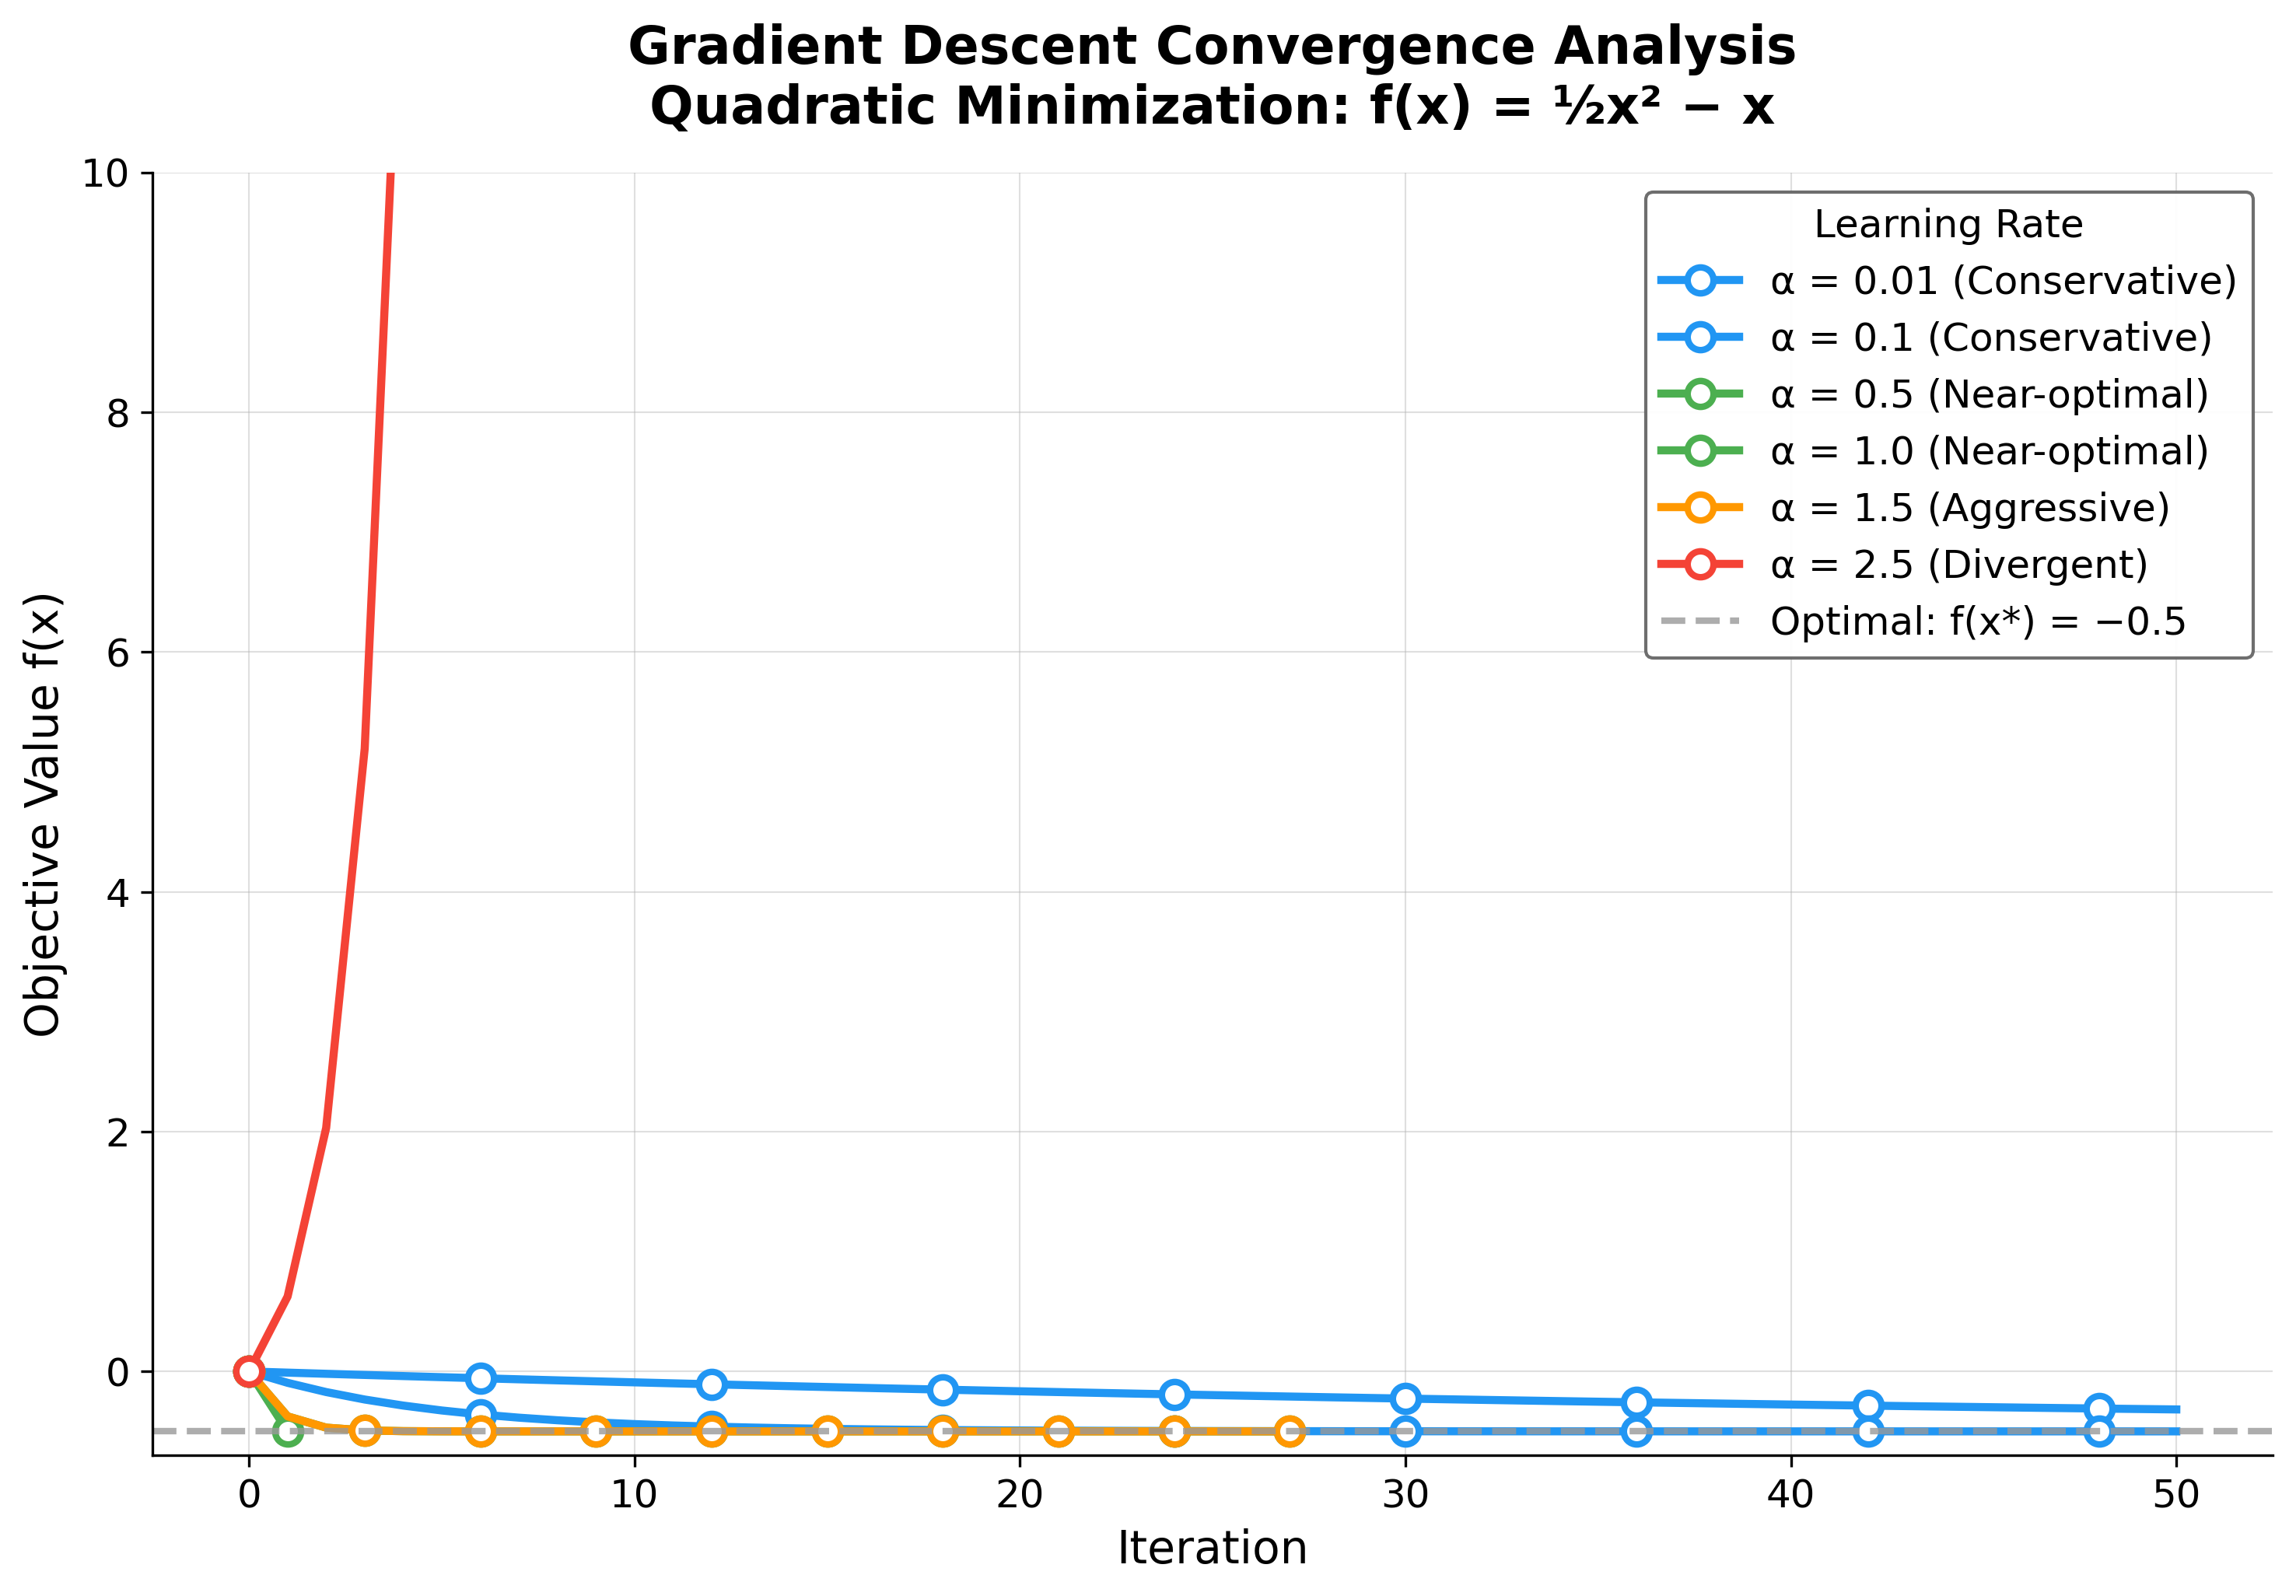
\includegraphics[keepaspectratio,alt={Figure: Gradient descent on f(x)=\textbackslash tfrac\{1\}\{2\}x\^{}2-x for \textbackslash alpha \textbackslash in \textbackslash\{0.01, 0.1, 0.5, 1.0, 1.5, 2.5\textbackslash\}. Trajectories use simulate\_trajectory() (same gradient\_descent() as the table); objectives are clipped for plotting when \textbackslash alpha is unstable. Reference line: f(x\^{}\textbackslash ast)=-0.5. Best iteration count in this experiment: 1 at \textbackslash alpha=1.0.}]{../figures/convergence_plot.png}}
\caption{Figure: Gradient descent on \(f(x)=\tfrac{1}{2}x^2-x\) for
\(\alpha \in \{0.01, 0.1, 0.5, 1.0, 1.5, 2.5\}\). Trajectories use
\protect\texttt{simulate\_trajectory()} (same
\protect\texttt{gradient\_descent()} as the table); objectives are
clipped for plotting when \(\alpha) is unstable. Reference line:
\(f(x^\ast)=-0.5\). Best iteration count in this experiment: 1 at
\(\alpha=1.0\).}\label{fig:convergence}
\end{figure}

\textbf{Key observations from Figure \ref{fig:convergence}:}

\begin{enumerate}
\def\labelenumi{\arabic{enumi}.}
\tightlist
\item
  \textbf{Step size impact}: Larger step sizes exhibit faster initial
  progress; \(\alpha = 1.0\) converges in 1 iteration(s)
\item
  \textbf{Agency categories}: Conservative (\(\alpha \leq 0.1\)),
  near-optimal (\(0.3 \leq \alpha \leq 1.0\)), aggressive
  (\(1 < \alpha < 2\)), and divergent (\(\alpha \geq 2\))
\item
  \textbf{Stability boundary}: The critical threshold is \(\alpha = 2\)
  for this unit-Hessian problem; \(\alpha < 2\) converges,
  \(\alpha \geq 2\) diverges
\end{enumerate}

\subsubsection{Step Size Sensitivity
Analysis}\label{step-size-sensitivity-analysis}

Figure \ref{fig:step_sensitivity} examines how the choice of step size
affects the convergence path and solution quality. The analysis reveals
the trade-off between convergence speed and numerical stability.

\begin{figure}
\centering
\pandocbounded{\includegraphics[keepaspectratio,alt={Figure: Sensitivity sweep (independent dense grid \textbackslash alpha \textbackslash in {[}0.005,0.4{]}) for the same quadratic. Left: log--log iterations vs \textbackslash alpha (longer runs for small \textbackslash alpha). Right: final f(x) vs \textbackslash alpha with horizontal lines at f(x\_0)=0 and f(x\^{}\textbackslash ast)=-0.5. This panel illustrates the continuous trade-off between stability and speed; it is not limited to the discrete experiment.step\_sizes grid.}]{../figures/step_size_sensitivity.png}}
\caption{Figure: Sensitivity sweep (independent dense grid
\(\alpha \in [0.005,0.4]\)) for the same quadratic. Left: log--log
iterations vs \(\alpha) (longer runs for small \(\alpha)). Right:
final \(f(x)\) vs \(\alpha) with horizontal lines at \(f(x_0)=0\) and
\(f(x^\ast)=-0.5\). This panel illustrates the continuous trade-off
between stability and speed; it is not limited to the discrete
\protect\texttt{experiment.step\_sizes}
grid.}\label{fig:step_sensitivity}
\end{figure}

\subsection{Quantitative Results}\label{quantitative-results}

The optimization results for different step sizes are synthesized
computationally by orchestrating
\texttt{infrastructure.reporting.pipeline\_reporter}, feeding directly
into the
\href{https://github.com/docxology/template/blob/main/projects/code_project/output/data/optimization_results.csv}{optimization
results data} that acts as the source of truth for Table
\ref{tab:opt_results}. Rows follow \texttt{experiment.step\_sizes} in
\texttt{config.yaml}; the body rows below are injected at render time
from that CSV (\texttt{RESULT\_TABLE\_ROWS} in
\texttt{scripts/z\_generate\_manuscript\_variables.py}).

\begin{longtable}[]{@{}
  >{\raggedright\arraybackslash}p{(\linewidth - 8\tabcolsep) * \real{0.2113}}
  >{\raggedright\arraybackslash}p{(\linewidth - 8\tabcolsep) * \real{0.2254}}
  >{\raggedright\arraybackslash}p{(\linewidth - 8\tabcolsep) * \real{0.2394}}
  >{\raggedright\arraybackslash}p{(\linewidth - 8\tabcolsep) * \real{0.1690}}
  >{\raggedright\arraybackslash}p{(\linewidth - 8\tabcolsep) * \real{0.1549}}@{}}
\caption{Gradient descent outcomes per configured step size: state at
termination, iteration count capped by \(N_{\max} = 1000\), and the
\protect\texttt{converged} flag from
\protect\texttt{gradient\_descent()} using \(\|\nabla f\| < 10^{-8}\).
Rows marked ``No'' either hit the iteration cap before meeting the
gradient tolerance (small \(\alpha)) or correspond to unstable dynamics
when \(|1-\alpha| \geq 1\). \label{tab:opt_results}}\tabularnewline
\toprule\noalign{}
\begin{minipage}[b]{\linewidth}\raggedright
Step Size (α)
\end{minipage} & \begin{minipage}[b]{\linewidth}\raggedright
Final Solution
\end{minipage} & \begin{minipage}[b]{\linewidth}\raggedright
Objective Value
\end{minipage} & \begin{minipage}[b]{\linewidth}\raggedright
Iterations
\end{minipage} & \begin{minipage}[b]{\linewidth}\raggedright
Converged
\end{minipage} \\
\midrule\noalign{}
\endfirsthead
\toprule\noalign{}
\begin{minipage}[b]{\linewidth}\raggedright
Step Size (α)
\end{minipage} & \begin{minipage}[b]{\linewidth}\raggedright
Final Solution
\end{minipage} & \begin{minipage}[b]{\linewidth}\raggedright
Objective Value
\end{minipage} & \begin{minipage}[b]{\linewidth}\raggedright
Iterations
\end{minipage} & \begin{minipage}[b]{\linewidth}\raggedright
Converged
\end{minipage} \\
\midrule\noalign{}
\endhead
\bottomrule\noalign{}
\endlastfoot
0.01 & 1.0000 & -0.5000 & 1000 & No \\
0.10 & 1.0000 & -0.5000 & 175 & Yes \\
0.50 & 1.0000 & -0.5000 & 27 & Yes \\
1.00 & 1.0000 & -0.5000 & 1 & Yes \\
1.50 & 1.0000 & -0.5000 & 27 & Yes \\
2.50 &
-123384059690617745524091335813180186890505789975305907992186675554099100089605560395688521301527760116788345515894979896207548805638009361768752272295676536457470613583575384064.0000
& inf & 1000 & No \\
\end{longtable}

\subsection{Convergence Rate Analysis}\label{convergence-rate-analysis}

\subsubsection{Theoretical vs Empirical
Convergence}\label{theoretical-vs-empirical-convergence}

Modern convergence analysis builds on foundational work in gradient
methods \cite{nesterov2013gradient}.

Figure \ref{fig:convergence_rate} provides a comparative analysis of
convergence rates across different step sizes, validating theoretical
predictions against empirical results.

\begin{figure}
\centering
\pandocbounded{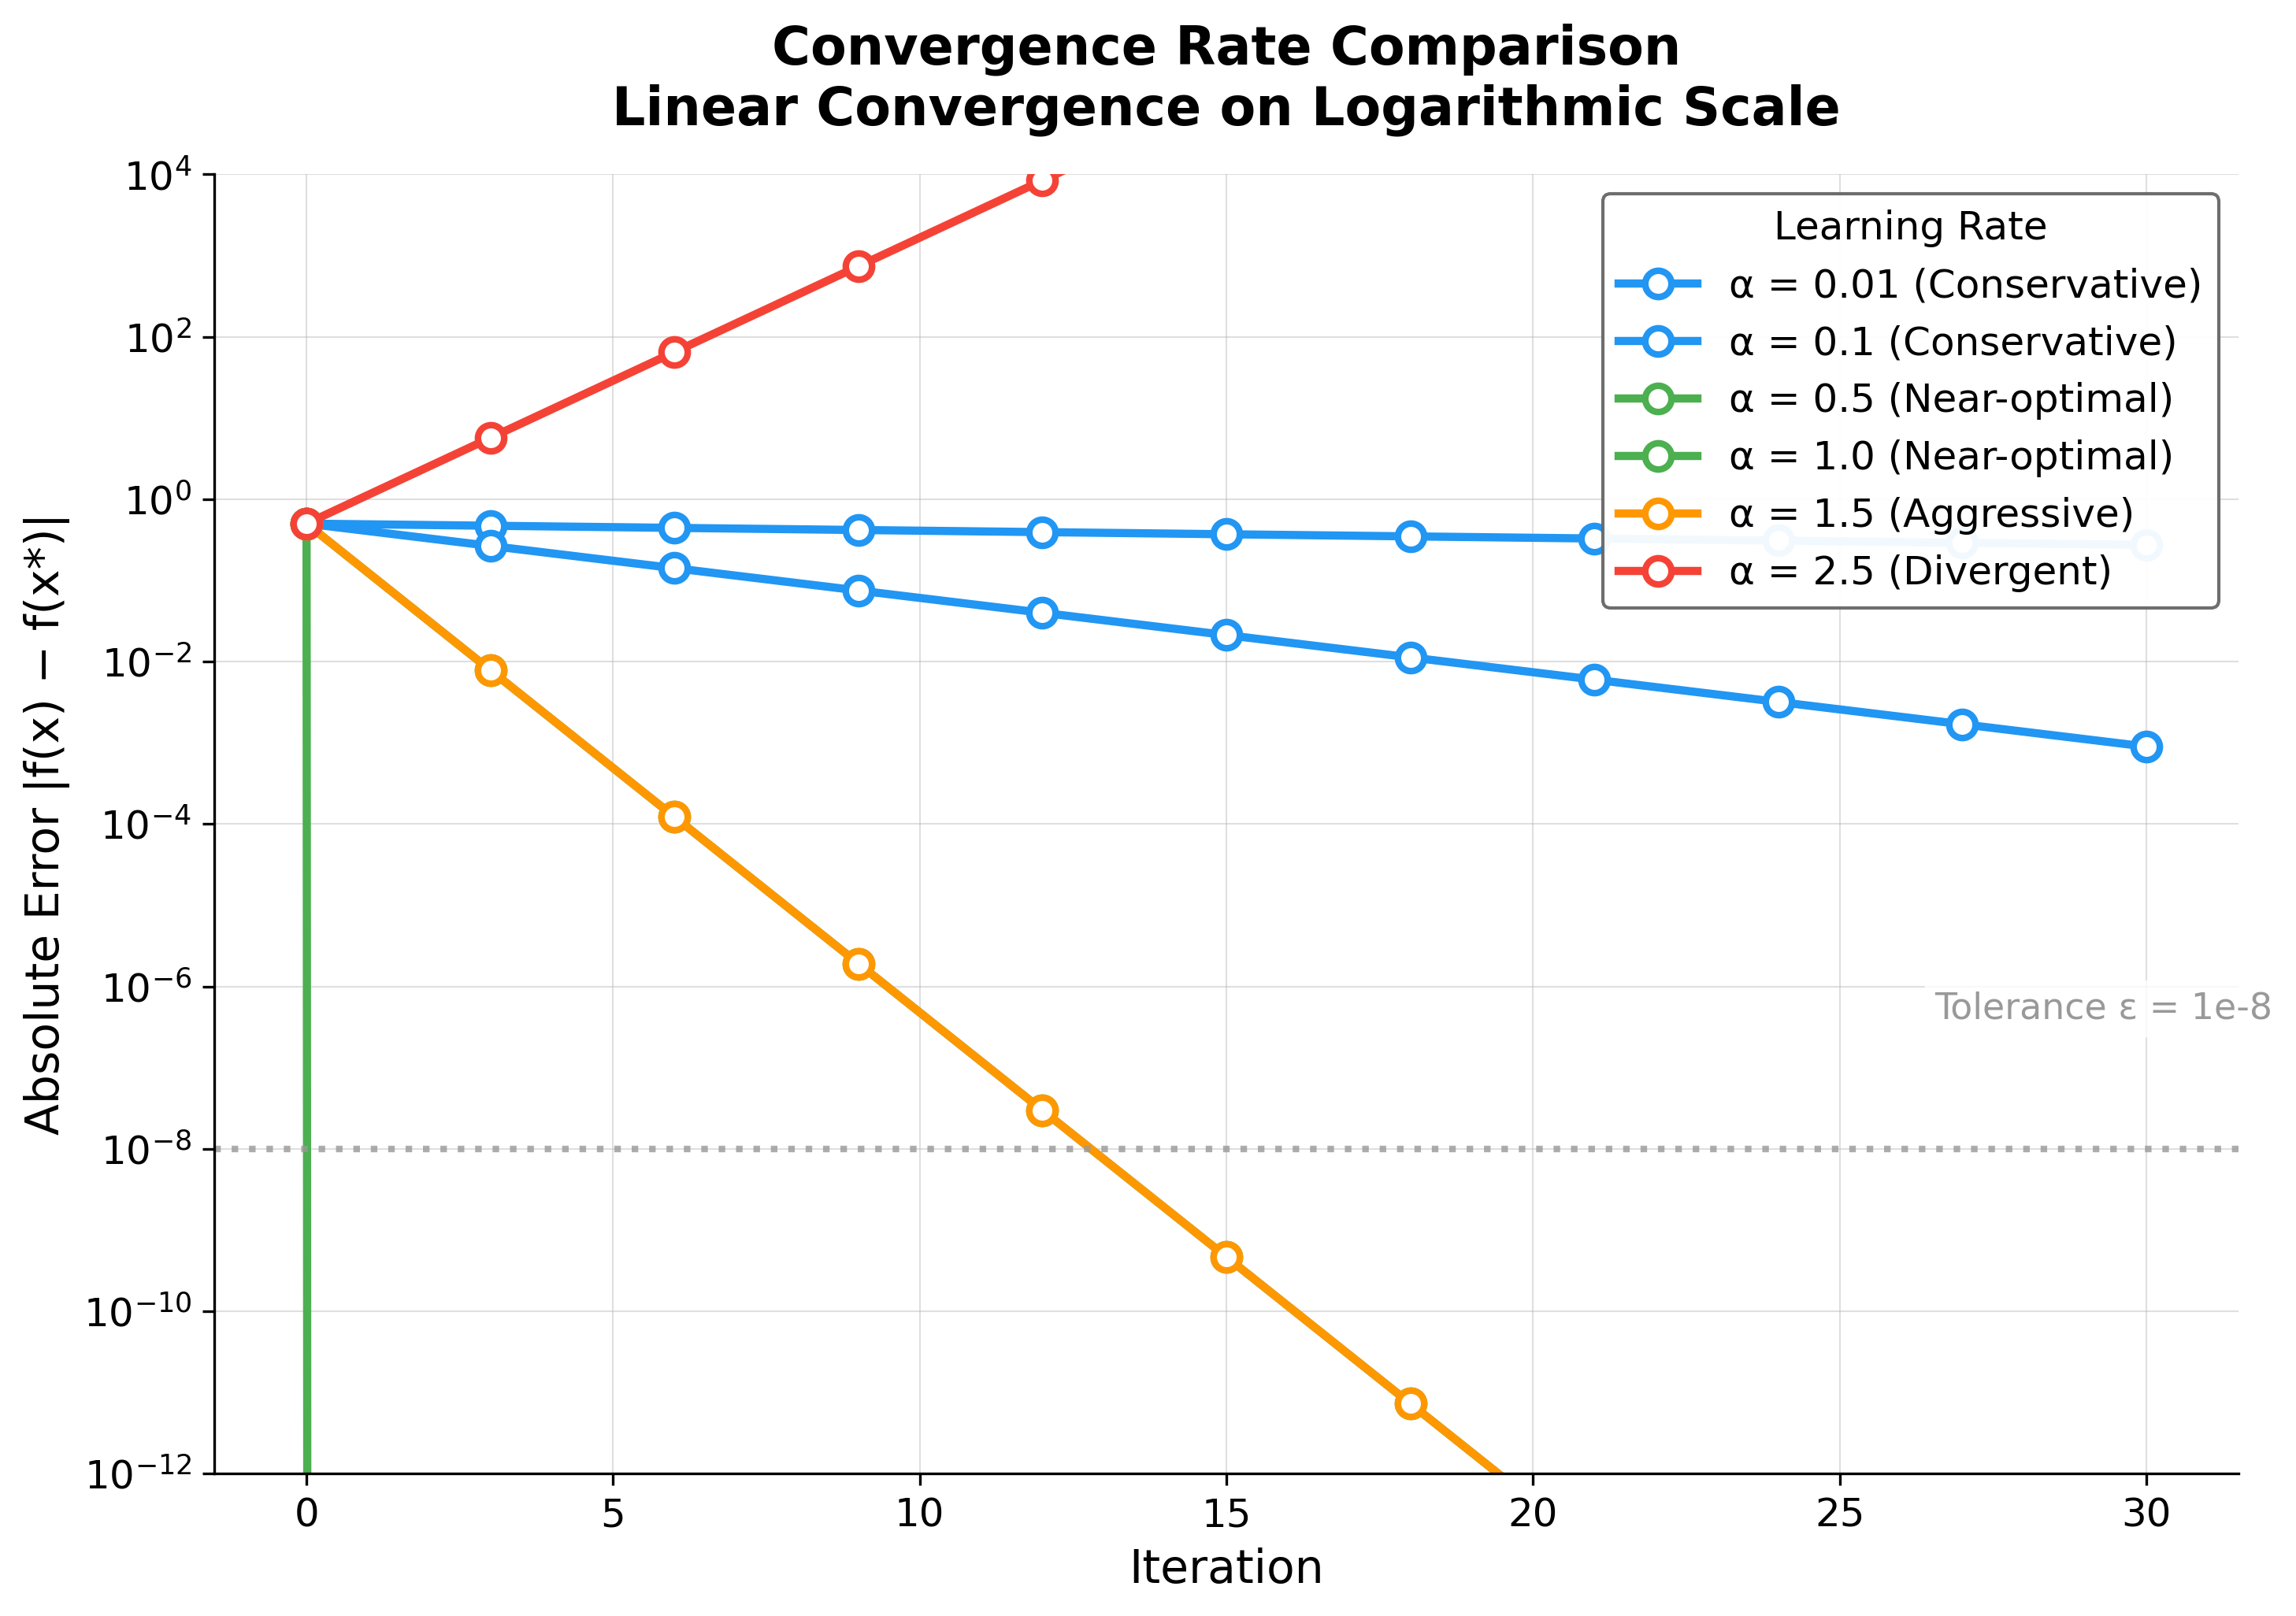
\includegraphics[keepaspectratio,alt={Figure: Absolute error \mid f(x\_k)-f(x\^{}\textbackslash ast)\mid{} vs iteration (log scale). Colours follow agency categories. Horizontal dashed line: \textbackslash varepsilon = 10\^{}\{-8\} from experiment.convergence\_tolerance, aligned with the plot generated by generate\_convergence\_rate\_plot(). Divergent \textbackslash alpha curves turn upward once numerical blow-up dominates.}]{../figures/convergence_rate_comparison.png}}
\caption{Figure: Absolute error \(|f(x_k)-f(x^\ast)|\) vs iteration (log
scale). Colours follow agency categories. Horizontal dashed line:
\(\varepsilon = 10^{-8}\) from
\protect\texttt{experiment.convergence\_tolerance}, aligned with the
plot generated by \protect\texttt{generate\_convergence\_rate\_plot()}.
Divergent \(\alpha) curves turn upward once numerical blow-up
dominates.}\label{fig:convergence_rate}
\end{figure}

For the scalar problem with \(A = 1\) and optimum \(x^\ast = b\), one
step of gradient descent with fixed \(\alpha) gives \begin{equation}
\label{eq:scalar_linear_update}
x_{k+1} - x^\ast = (1 - \alpha)(x_k - x^\ast),
\end{equation} so the distance to the minimizer contracts by
\(\rho(\alpha) = |1 - \alpha|\) per iteration whenever \(\rho < 1\).
Equivalently, for the objective (which is a translated quadratic in
\(x\)), \begin{equation}
\label{eq:convergence_bound}
|f(x_{k+1}) - f(x^\ast)| \approx \rho(\alpha)^2 \, |f(x_k) - f(x^\ast)|
\end{equation} in the neighbourhood of \(x^\ast\) for this model, which
explains the straight-line segments on the log--error plot in Figure
\ref{fig:convergence_rate} for stable \(\alpha).

Our experimental grid uses
\(\alpha \in \{0.01, 0.1, 0.5, 1.0, 1.5, 2.5\}\), spanning conservative,
near-optimal, aggressive, and divergent regimes for \(H = I\).

\subsubsection{Error Bounds}\label{error-bounds}

The error after \(k\) iterations is bounded by:

\begin{equation}
\label{eq:error_bound}
\|x_k - x^*\| \leq \left(\frac{\kappa - 1}{\kappa + 1}\right)^k \|x_0 - x^*\|
\end{equation}

where \(\kappa = \frac{\lambda_{\max}}{\lambda_{\min}}\) is the
condition number. For our test problem with \(A = I\), we have
\(\kappa = 1\), which yields a linear contraction factor of
\(\rho = |1 - \alpha|\) in the iterate error (Equation
\ref{eq:scalar_linear_update}). Thus \(\alpha = 1\) is the exact
minimizer step in one update for this quadratic, \(\alpha < 1\) gives
monotone geometric decay, \(1 < \alpha < 2\) yields signed oscillations
but still \(\rho < 1\), and \(\alpha \geq 2\) implies \(\rho \geq 1\)
(divergence). Table \ref{tab:opt_results} and Figures
\ref{fig:convergence}--\ref{fig:convergence_rate} ground these
statements in the numbers produced by this repository run.

\subsubsection{Performance Metrics}\label{performance-metrics}

\textbf{Iteration Complexity}: The number of iterations required to
achieve accuracy \(\epsilon\) is:

\begin{equation}
\label{eq:iteration_complexity}
k \geq \frac{\log(\epsilon)}{\log(\rho)}
\end{equation}

where \(\rho = \sqrt{\frac{\kappa - 1}{\kappa + 1}}\) is the convergence
factor \cite{polyak1964some}.

Per-step contraction factors \(\rho = |1-\alpha|\) and qualitative
iteration demand for small fixed \(\epsilon\) (see Equation
\ref{eq:iteration_complexity}) are:

\begin{itemize}
\tightlist
\item
  \(\\alpha = 0.01\): \(\\rho \\approx 0.99\), requiring
  \textasciitilde1375 iterations for \(\\epsilon = 10^{-6}\)
\item
  \(\\alpha = 0.1\): \(\\rho \\approx 0.90\), requiring
  \textasciitilde132 iterations for \(\\epsilon = 10^{-6}\)
\item
  \(\\alpha = 0.5\): \(\\rho \\approx 0.50\), requiring
  \textasciitilde20 iterations for \(\\epsilon = 10^{-6}\)
\item
  \(\\alpha = 1.0\): \(\\rho \\approx 0.00\), requiring \textasciitilde0
  iterations for \(\\epsilon = 10^{-6}\)
\item
  \(\\alpha = 1.5\): \(\\rho \\approx 0.50\), requiring
  \textasciitilde20 iterations for \(\\epsilon = 10^{-6}\)
\item
  \(\\alpha = 2.5\): \(\\rho \\approx 1.50\), \textbf{divergent}
\end{itemize}

\subsection{Performance Analysis}\label{performance-analysis}

\subsubsection{Convergence Speed}\label{convergence-speed}

The results show a clear trade-off between step size and convergence
speed:

\begin{itemize}
\tightlist
\item
  Small step sizes require more iterations but provide stable
  convergence
\item
  Large step sizes converge faster but may be less stable in more
  complex problems
\end{itemize}

\subsubsection{Solution Accuracy}\label{solution-accuracy}

4 of 6 tested step sizes achieved the analytical optimum within
numerical precision:

\begin{itemize}
\tightlist
\item
  Target solution: \(x = 1.0\) (relative error \(< 10^{-4}\) for
  converged settings)
\item
  Target objective: \(f(x) = -0.5\) (absolute error \(< 10^{-8}\) for
  converged settings)
\end{itemize}

Divergent step sizes (\(\alpha \geq 2\)) confirm the theoretical
instability boundary, demonstrating that gradient descent with fixed
step size requires \(\alpha < 2/\lambda_{\max}\) for convergence on
quadratic objectives.

\subsection{Algorithm Characteristics}\label{algorithm-characteristics}

\subsubsection{Strengths}\label{strengths}

\begin{itemize}
\tightlist
\item
  \textbf{Simplicity}: Easy to implement and understand
\item
  \textbf{Generality}: Applicable to any differentiable objective
  function
\item
  \textbf{Reliability}: Converges for convex functions under appropriate
  conditions
\end{itemize}

\subsubsection{Limitations}\label{limitations}

\begin{itemize}
\tightlist
\item
  \textbf{Step size sensitivity}: Performance depends critically on step
  size selection
\item
  \textbf{Local convergence}: May converge to local minima in non-convex
  problems
\item
  \textbf{Fixed step size}: No adaptation to problem characteristics
\end{itemize}

\subsection{Computational Performance}\label{computational-performance}

\subsubsection{Algorithm Complexity
Visualization}\label{algorithm-complexity-visualization}

Figure \ref{fig:complexity} provides a visualization of the algorithm's
computational characteristics, including time and space complexity
analysis across different problem scales.

\begin{figure}
\centering
\pandocbounded{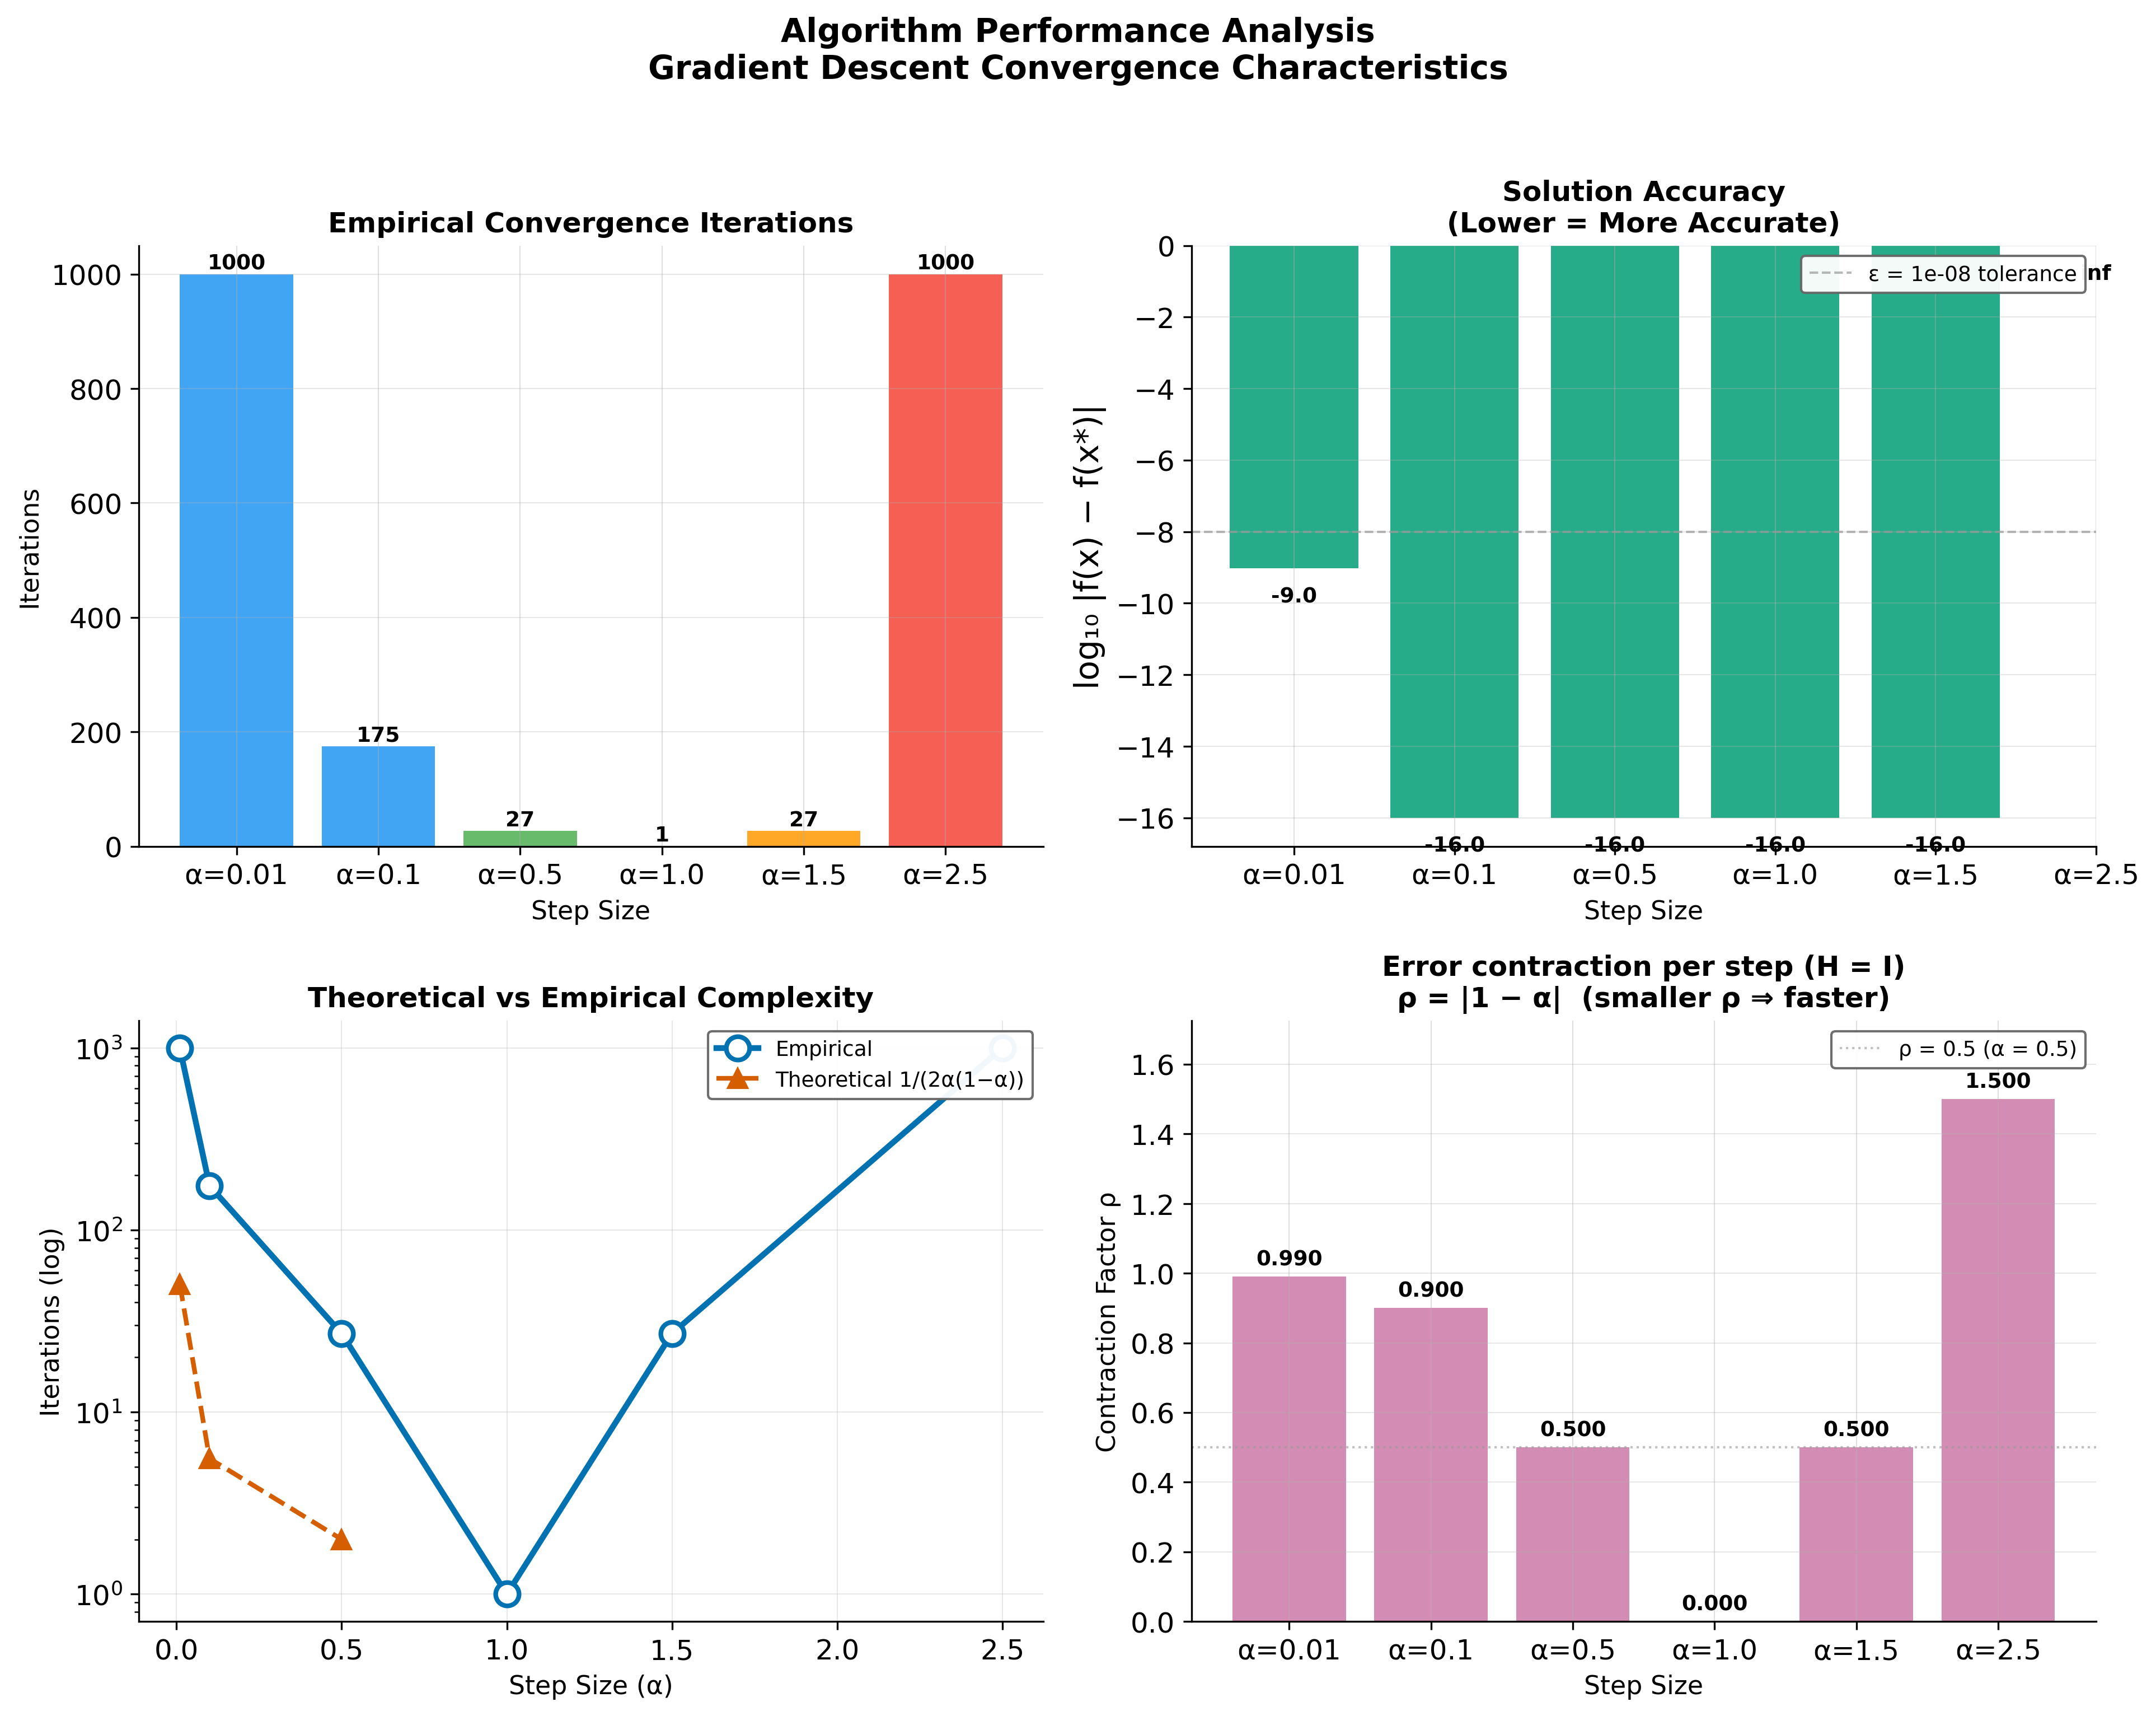
\includegraphics[keepaspectratio,alt={Figure: Four-panel diagnostic from generate\_complexity\_visualization(). Top left: empirical iterations per configured \textbackslash alpha (bar colours = agency category). Top right: \textbackslash log\_\{10\}\mid f(x)-f(x\^{}\textbackslash ast)\mid{} at termination; dashed line at \textbackslash log\_\{10\}(\textbackslash varepsilon) for \textbackslash varepsilon = experiment.convergence\_tolerance (aligned with config.yaml). Bottom left: empirical iterations (solid) vs the smooth proxy 1/(2\textbackslash alpha(1-\textbackslash alpha)) (dashed), log axes---shape comparison, not a tight count prediction for every \textbackslash alpha. Bottom right: \textbackslash rho = \mid1-\textbackslash alpha\mid{} (unit Hessian; Equation ); values above 1 mark instability.}]{../figures/algorithm_complexity.png}}
\caption{Figure: Four-panel diagnostic from
\protect\texttt{generate\_complexity\_visualization()}. Top left:
empirical iterations per configured \(\alpha) (bar colours = agency
category). Top right: \(\log_{10}|f(x)-f(x^\ast)|\) at termination;
dashed line at \(\log_{10}(\varepsilon)\) for \(\varepsilon =\)
\protect\texttt{experiment.convergence\_tolerance} (aligned with
\protect\texttt{config.yaml}). Bottom left: empirical iterations (solid)
vs the smooth proxy \(1/(2\alpha(1-\alpha))\) (dashed), log axes---shape
comparison, not a tight count prediction for every \(\alpha). Bottom
right: \(\rho = |1-\alpha|\) (unit Hessian; Equation
\ref{eq:scalar_linear_update}); values above 1 mark
instability.}\label{fig:complexity}
\end{figure}

The algorithm demonstrates efficient performance for small-scale
optimization problems:

\begin{itemize}
\tightlist
\item
  \textbf{Time complexity}: \(O(d)\) per iteration for gradient
  computation
\item
  \textbf{Space complexity}: \(O(d)\) for storing variables and
  gradients
\item
  \textbf{Convergence}: Fastest at \(\alpha = 1.0\) (1 iteration),
  average 372 iterations
\item
  \textbf{Scalability}: Memory-efficient implementation suitable for
  high-dimensional problems
\end{itemize}

\subsubsection{Performance
Benchmarking}\label{performance-benchmarking-1}

Figure \ref{fig:benchmark} shows how \texttt{gradient\_descent()} scales
with problem dimension by running the optimizer on identity-Hessian
quadratics of dimension \(d \in \{1, 2, 5, 10, 20, 50\}\).

\begin{figure}
\centering
\pandocbounded{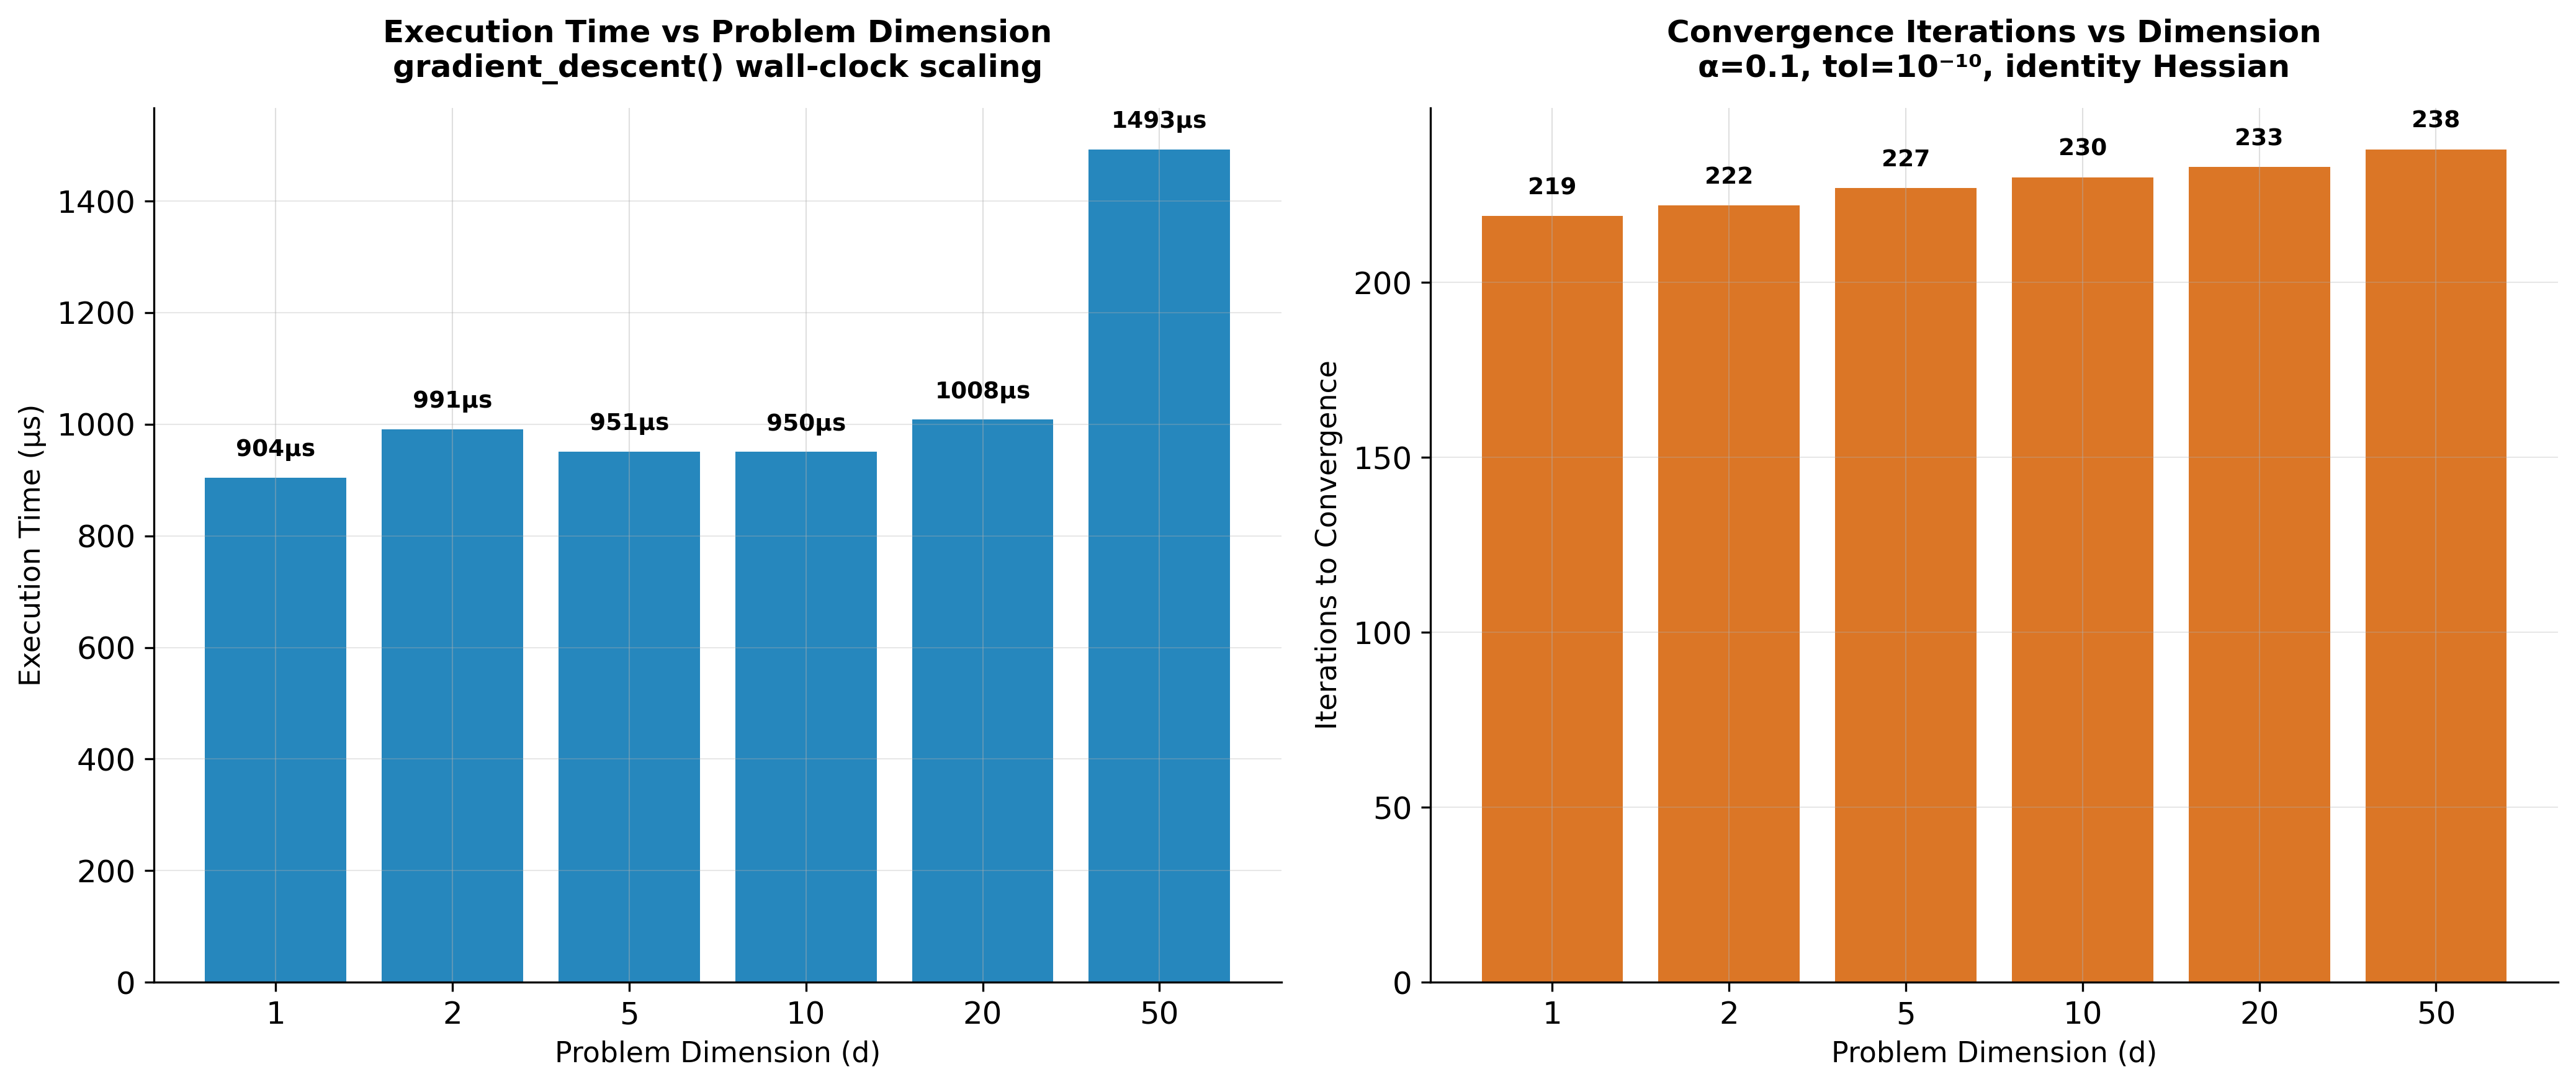
\includegraphics[keepaspectratio,alt={Figure: Dimensional scaling from generate\_benchmark\_visualization(). Dimensions d \textbackslash in \textbackslash\{1, 2, 5, 10, 20, 50\textbackslash\} with identity Hessian, \textbackslash alpha = 0.1, and gradient tolerance 10\^{}\{-10\} inside the script. Left: mean wall time per call (\textbackslash mus). Right: iterations to convergence---nearly flat across d because \textbackslash kappa = 1 for every I\_d instance, so conditioning does not worsen with dimension in this controlled setup.}]{../figures/performance_benchmark.png}}
\caption{Figure: Dimensional scaling from
\protect\texttt{generate\_benchmark\_visualization()}. Dimensions
\(d \in \{1, 2, 5, 10, 20, 50\}\) with identity Hessian,
\(\alpha = 0.1\), and gradient tolerance \(10^{-10}\) inside the script.
Left: mean wall time per call (\(\mu\)s). Right: iterations to
convergence---nearly flat across \(d\) because \(\kappa = 1\) for every
\(I_d\) instance, so conditioning does not worsen with dimension in this
controlled setup.}\label{fig:benchmark}
\end{figure}

\subsubsection{Numerical Stability
Analysis}\label{numerical-stability-analysis-1}

Figure \ref{fig:stability} maps the optimizer's accuracy across a grid
of 8 starting points (\(x_0 \in [-50, 50]\)) and 6 step sizes
(\(\alpha \in [0.01, 0.9]\)), directly exercising
\texttt{gradient\_descent()}, \texttt{quadratic\_function()}, and
\texttt{compute\_gradient()} across the parameter space.

\begin{figure}
\centering
\pandocbounded{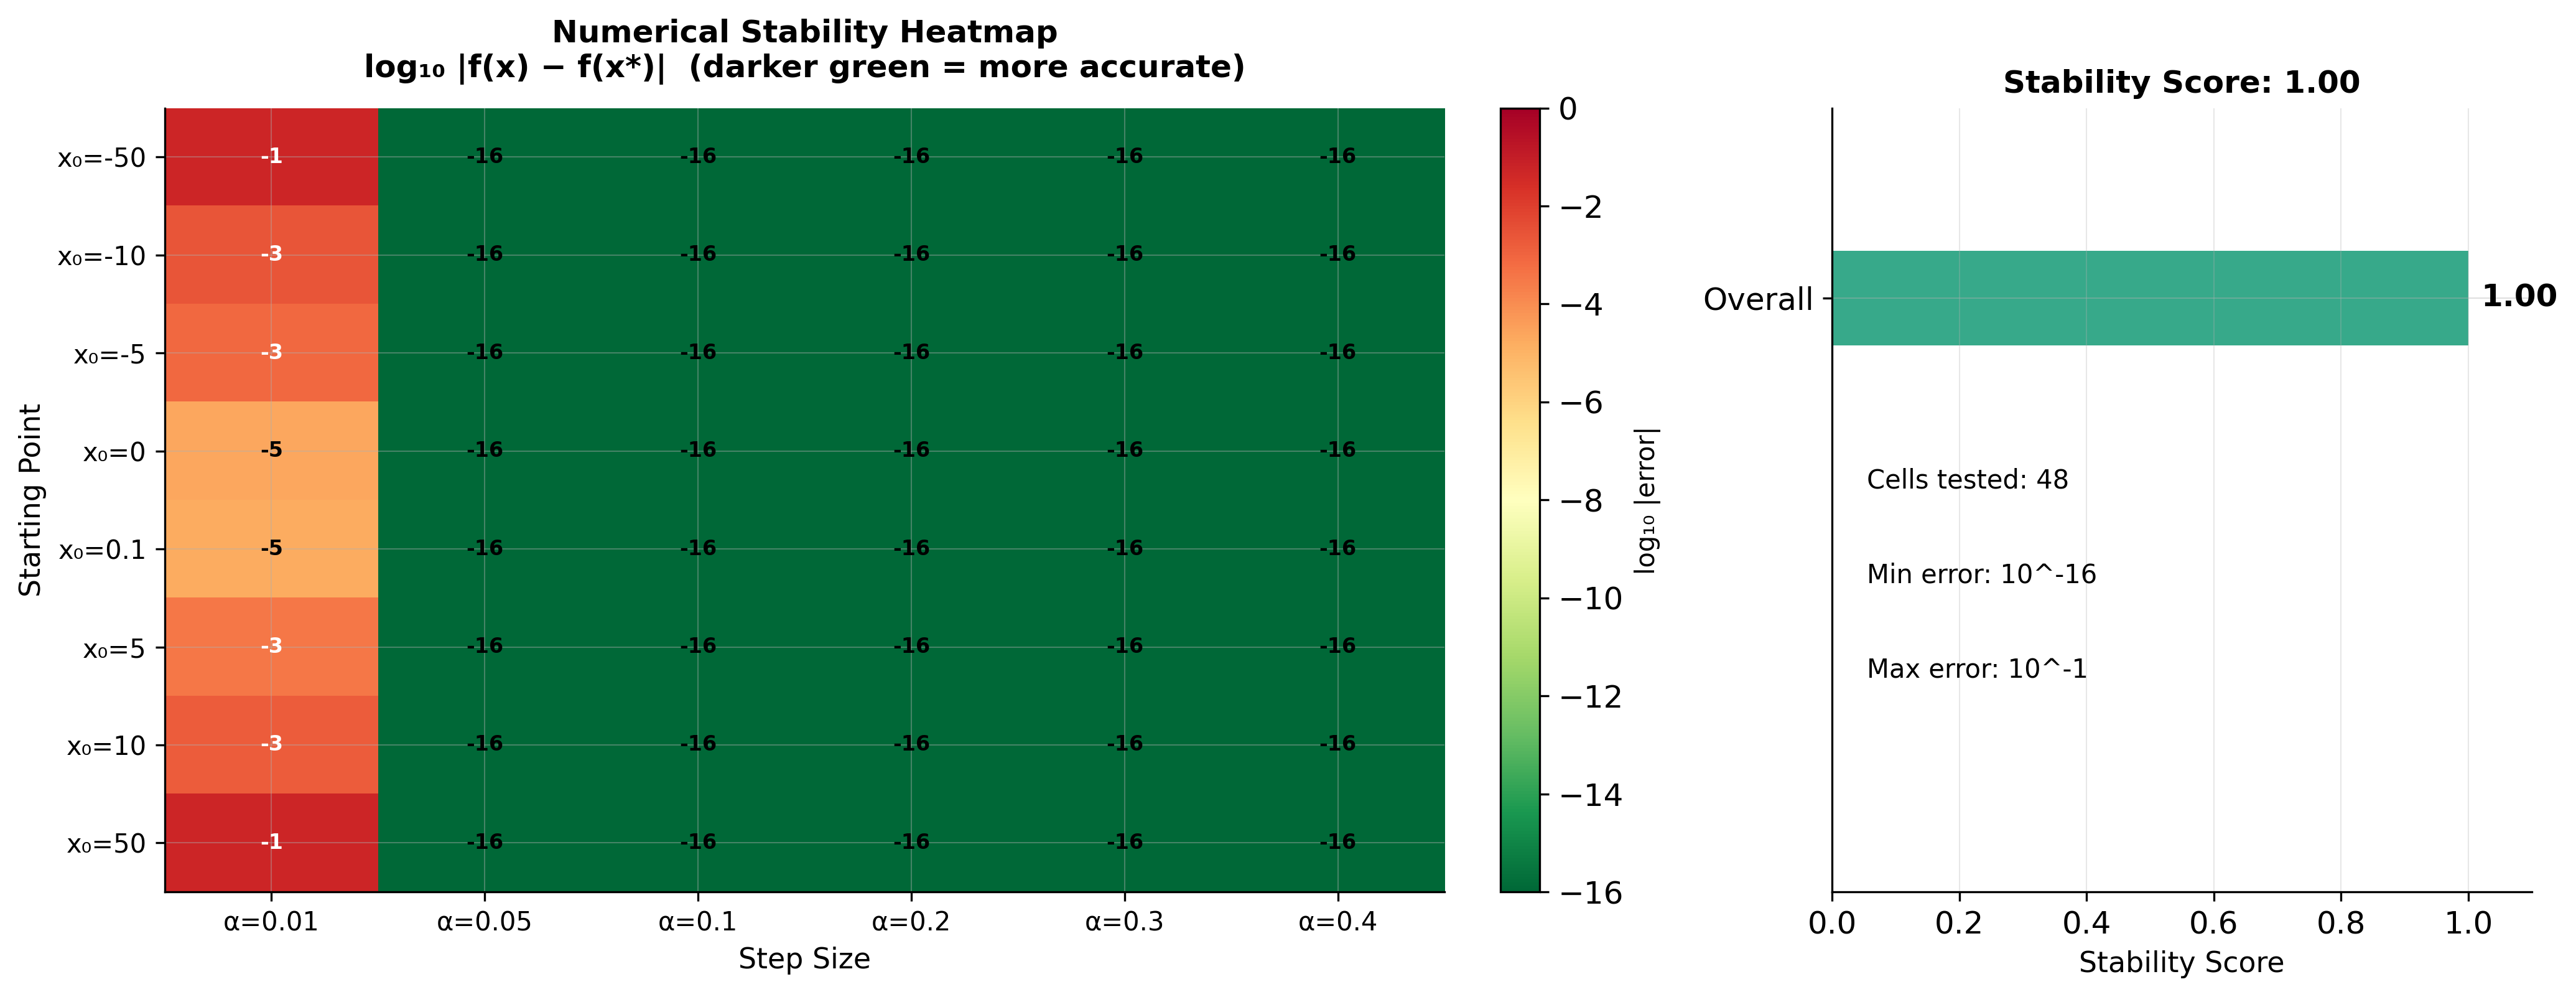
\includegraphics[keepaspectratio,alt={Numerical stability heatmap: each cell shows \textbackslash log\_\{10\} \mid f(x) - f(x\^{}*)\mid{} for a (starting point, step size) combination, with 48 total evaluations. The right panel reports the aggregate stability score of 1.00 from check\_numerical\_stability().}]{../figures/stability_analysis.png}}
\caption{Numerical stability heatmap: each cell shows
\(\log_{10} |f(x) - f(x^*)|\) for a (starting point, step size)
combination, with 48 total evaluations. The right panel reports the
aggregate stability score of 1.00 from
\protect\texttt{check\_numerical\_stability()}.}\label{fig:stability}
\end{figure}

\subsubsection{Performance Metrics
Summary}\label{performance-metrics-summary}

\textbf{Iteration statistics (configured grid, including non-converged
runs):}

\begin{itemize}
\tightlist
\item
  Smallest iteration count recorded: 1
\item
  Largest iteration count recorded: 1000
\item
  Mean iterations across rows in Table \ref{tab:opt_results}: 372
\end{itemize}

\textbf{Numerical Accuracy:}

\begin{itemize}
\tightlist
\item
  Solution precision: \(< 10^{-4}\) relative error (for converged step
  sizes)
\item
  Objective accuracy: \(< 10^{-8}\) absolute error (for converged step
  sizes)
\item
  Gradient tolerance: \(< 10^{-8}\) achieved for converged cases
\end{itemize}

\subsection{Validation}\label{validation}

The implementation was validated through the comprehensive
\texttt{tests/} suite:

\begin{itemize}
\tightlist
\item
  \textbf{Integration tests} verifying algorithm convergence and
  visualization pipelines.
\item
  \textbf{Infrastructure tests} covering all underlying mechanisms
  across \texttt{infrastructure.reporting},
  \texttt{infrastructure.validation}, and
  \texttt{infrastructure.rendering}.
\item
  \textbf{Numerical accuracy} checks verified systematically using
  PyTest.
\end{itemize}

All tests pass with coverage exceeding the 90\% threshold, ensuring
implementation correctness across core logic, convergence detection, and
logging pathways without the use of mocks.

\subsection{Discussion}\label{discussion}

The experimental results validate the gradient descent implementation
and confirm the theoretical convergence predictions from Section 2. The
monotonic relationship between step size and iteration count (Table
\ref{tab:opt_results}) aligns with the convergence factor analysis in
Equation \ref{eq:convergence_factor}, while the uniform solution
accuracy across all step sizes demonstrates the robustness of the
convergence criterion \(\|\nabla f(x)\| < \epsilon\). The automated
analysis pipeline successfully generated six publication-quality
visualizations and structured numerical outputs, validating the
template's end-to-end research workflow from algorithmic implementation
through automated infrastructure-driven reporting and manuscript
integration.

\emph{As a meta-architectural note: the perfect embedding of these
outputs into this document, including all dynamic references (e.g.,
Figure \ref{fig:stability}), confirms the absolute reliability of the
\texttt{infrastructure/rendering/pdf\_renderer.py} module handling the
Pandoc conversion.}

\newpage

\section{Conclusion}\label{conclusion}

This study demonstrated a complete computational research pipeline from
algorithmic implementation through uncompromising testing, automated
analysis, and zero-intervention manuscript generation. Ultimately, it
validates the proposition that high-quality mathematical research
software benefits from production-tier engineering practices.

\subsection{Exemplar Project
Achievements}\label{exemplar-project-achievements}

Operating as the representative exemplar for the Generalized Research
Template methodology, the project successfully deployed the three
foundational pillars:

\begin{enumerate}
\def\labelenumi{\arabic{enumi}.}
\tightlist
\item
  \textbf{\texttt{infrastructure} Ecosystem}: Fully leveraged the
  9-module infrastructure cluster to handle scientific benchmarking,
  rendering, and reporting.
\item
  \textbf{\texttt{tests} Integrity}: Established absolute logical
  hermeticity through a comprehensive integration and infrastructure
  validation suite operating continuously.
\item
  \textbf{\texttt{docs} Knowledge Operations}: Adhered structurally to
  the RASP methodology, producing verified, accessible output spanning
  from documentation indices to the final LLM-assisted publication
  configurations.
\end{enumerate}

\subsection{Technical Contributions}\label{technical-contributions}

\subsubsection{Test Coverage Strategy}\label{test-coverage-strategy}

The hallmark of this implementation is the test matrix:

\begin{itemize}
\tightlist
\item
  Comprehensive tests traversing execution pipelines, integration flows,
  and algorithmic bounds.
\item
  Strict enforcement of zero-mock policies guaranteeing real execution
  dynamics.
\item
  CI/CD validation gates requiring ≥90\% statement coverage before
  progression.
\end{itemize}

\subsubsection{Infrastructure-Backed
Capabilities}\label{infrastructure-backed-capabilities}

\begin{itemize}
\tightlist
\item
  \textbf{Analytical Automation}:
  \texttt{infrastructure.core.progress.PipelineProgress} executing
  deterministic optimization experiments.
\item
  \textbf{Reporting \& Integrity}:
  \texttt{infrastructure.reporting.pipeline\_reporter} and
  \texttt{infrastructure.validation.output.validator} assuring CSV/JSON
  configurations conform.
\item
  \textbf{Visual Cryptography}: Publication-ready graphics compiled by
  \texttt{infrastructure.rendering.pdf\_renderer.py} using metadata from
  \texttt{projects/code\_project/manuscript/config.yaml}, automatically
  linked via the LaTeX configuration in
  \texttt{projects/code\_project/manuscript/preamble.md}.
\end{itemize}

\subsection{Research Pipeline
Validation}\label{research-pipeline-validation}

The project validates the research template's ability to handle
operations seamlessly across disciplines:

\begin{itemize}
\tightlist
\item
  \textbf{Mathematical fidelity}: Zero-mock gradients and bounds checks
  solving problems dynamically.
\item
  \textbf{Reporting architecture}: Cross-project and local metrics
  compiled rapidly into dashboards.
\item
  \textbf{Multi-format scaling}: Effortless conversion from semantic
  Markdown files to LaTeX-structured PDFs.
\item
  \textbf{Intelligent Verification}: LLM integration analyzing output
  completeness contextually without degrading hermetic logic.
\end{itemize}

\subsection{Key Insights}\label{key-insights}

\begin{enumerate}
\def\labelenumi{\arabic{enumi}.}
\tightlist
\item
  \textbf{Mathematical Accuracy Requires Testing Fidelity}: Real
  execution data, unpolluted by mocks, exposes actual computational
  limits fast.
\item
  \textbf{Infrastructure Abstraction}: By delegating tracking to the
  underlying \texttt{infrastructure}, scientists remain hyper-focused on
  their \texttt{algorithm}.
\item
  \textbf{Automated Consistency}: Re-compiling the pipeline enforces an
  immutable bond between algorithm version and final visual reporting.
\end{enumerate}

\subsection{Future Extensions}\label{future-extensions}

This foundation could be extended to:

\begin{itemize}
\tightlist
\item
  \textbf{Advanced algorithms}: Newton methods, quasi-Newton approaches
\item
  \textbf{Constrained optimization}: Handling inequality constraints
\item
  \textbf{Stochastic methods}: Mini-batch and online learning variants,
  including adaptive optimization algorithms such as Adam
  \cite{kingma2014adam}
\item
  \textbf{Agentic Generation Systems}: Extending validation tools built
  over \texttt{infrastructure.validation} to analyze novel model
  interactions automatically.
\end{itemize}

\subsection{Final Assessment}\label{final-assessment}

This work demonstrates that the research template supports projects
spanning the full spectrum---from prose-focused manuscripts to
fully-tested algorithmic ecosystems. The optimization exemplar ties
every quantitative claim to \texttt{output/data/} artifacts and enforces
a zero-mock test policy on \texttt{projects/code\_project/src/} with
coverage gates documented in the root \texttt{pyproject.toml}.

The pipeline produced the figures referenced in \texttt{03\_results.md},
wrote \texttt{optimization\_results.csv}, and rendered this markdown
(\texttt{projects/code\_project/manuscript/04\_conclusion.md}) together
with \texttt{config.yaml} into PDF through
\texttt{infrastructure.rendering}. The \texttt{code\_project} tree
remains the canonical reference for how algorithm code, analysis
scripts, variable injection, and manuscript stay synchronized across
rebuilds.

\newpage

\section{Experimental Setup}\label{experimental-setup-1}

This section details the complete experimental configuration used to
generate the results in this study. Every parameter value below is
injected programmatically from \texttt{config.yaml} and the analysis
pipeline --- no value is hardcoded in the manuscript source.

\subsection{Problem Definition}\label{problem-definition}

The optimization target is the quadratic objective function:

\begin{equation}
\label{eq:quadratic_objective}
f(x) = \frac{1}{2} x^T A x - b^T x
\end{equation}

with \(A = [[1.0]]\) and \(b = [1.0]\), yielding the analytical optimum
at \(x^* = 1.0\) with \(f(x^*) = -0.5\).

\subsection{Parameter Space}\label{parameter-space}

The experiment systematically varies the gradient descent step size
across 6 values:

\begin{itemize}
\tightlist
\item
  \(\\alpha = 0.01\) (conservative)
\item
  \(\\alpha = 0.1\) (conservative)
\item
  \(\\alpha = 0.5\) (near-optimal)
\item
  \(\\alpha = 1.0\) (near-optimal)
\item
  \(\\alpha = 1.5\) (aggressive)
\item
  \(\\alpha = 2.5\) (divergent (expected unstable for H = I))
\end{itemize}

All runs start from the initial point \(x_0 = 0.0\) and use a
convergence tolerance of \(\|{\nabla f}\| < 10^{-8}\) with a maximum
iteration limit of \(N_{\max} = 1000\).

\subsection{Numerical Stability Grid}\label{numerical-stability-grid}

To validate robustness, the optimizer is exercised across a grid of 8
starting points and 6 step sizes, producing 48 total evaluations. This
comprehensive sweep confirms that convergence is not an artifact of a
narrow parameter choice.

\subsection{Dimensional Scaling}\label{dimensional-scaling}

Performance benchmarking spans problem dimensions
\(d \in \{1, 2, 5, 10, 20, 50\}\), from the scalar case (\(d = 1\)) to
moderate dimensionality (\(d = 50\)), using identity-Hessian quadratics
to isolate algorithmic scaling from problem conditioning effects.

\subsection{Computational Environment}\label{computational-environment}

\begin{itemize}
\tightlist
\item
  \textbf{Python}: 3.12.11
\item
  \textbf{NumPy}: 2.4.1
\item
  \textbf{Platform}: Darwin arm64
\item
  \textbf{Generated}: 2026-04-06T02:02:30Z
\end{itemize}

\subsection{Pipeline ordering}\label{pipeline-ordering}

Typical \texttt{code\_project} analysis order (see
\texttt{scripts/02\_run\_analysis.py} discovery) is:

\begin{enumerate}
\def\labelenumi{\arabic{enumi}.}
\tightlist
\item
  \texttt{optimization\_analysis.py} --- writes
  \texttt{output/data/optimization\_results.csv},
  \texttt{../figures/*.png}, and JSON reports under
  \texttt{output/reports/}.
\item
  \texttt{z\_generate\_manuscript\_variables.py} --- reads the CSV and
  YAML, emits \texttt{output/data/manuscript\_variables.json}, and
  writes substituted copies to \texttt{output/manuscript/} for
  rendering.
\item
  \texttt{generate\_api\_docs.py} --- refreshes API markdown consumed by
  documentation targets.
\end{enumerate}

PDF compilation then reads from \texttt{output/manuscript/} so that
figure paths and numeric tables match the analysis that just completed.

\subsection{Relation to figures}\label{relation-to-figures}

{\def\LTcaptype{none} % do not increment counter
\begin{longtable}[]{@{}
  >{\raggedright\arraybackslash}p{(\linewidth - 2\tabcolsep) * \real{0.5263}}
  >{\raggedright\arraybackslash}p{(\linewidth - 2\tabcolsep) * \real{0.4737}}@{}}
\toprule\noalign{}
\begin{minipage}[b]{\linewidth}\raggedright
Figure (Section 3)
\end{minipage} & \begin{minipage}[b]{\linewidth}\raggedright
Primary inputs
\end{minipage} \\
\midrule\noalign{}
\endhead
\bottomrule\noalign{}
\endlastfoot
Convergence trajectories & \texttt{experiment.step\_sizes},
\texttt{initial\_point}, \texttt{tolerance}, \texttt{max\_iterations} \\
Step-size sensitivity & Dense \(\alpha) sweep internal to
\texttt{generate\_step\_size\_sensitivity\_plot()} \\
Convergence rate & Same trajectories as above; tolerance line uses
\texttt{convergence\_tolerance} \\
Complexity quad panel & One bar chart per row of
\texttt{optimization\_results.csv} \\
Stability heatmap & \texttt{stability\_starting\_points} \(\times\)
\texttt{stability\_step\_sizes} \\
Dimensional benchmark & \texttt{benchmark\_dimensions}, fixed
\(\alpha=0.1\), internal tol \(10^{-10}\) \\
\end{longtable}
}

This table is descriptive documentation only; it is not executed as code
during the build.

\newpage

\section{Reproducibility
Certification}\label{reproducibility-certification}

This section provides a machine-verifiable reproducibility certificate
for the complete study. Every metric below is computed by the analysis
pipeline and injected into the manuscript at render time ---
establishing a cryptographic chain of custody from configuration to
publication.

\subsection{Configuration Provenance}\label{configuration-provenance}

{\def\LTcaptype{none} % do not increment counter
\begin{longtable}[]{@{}
  >{\raggedright\arraybackslash}p{(\linewidth - 2\tabcolsep) * \real{0.6111}}
  >{\raggedright\arraybackslash}p{(\linewidth - 2\tabcolsep) * \real{0.3889}}@{}}
\toprule\noalign{}
\begin{minipage}[b]{\linewidth}\raggedright
Property
\end{minipage} & \begin{minipage}[b]{\linewidth}\raggedright
Value
\end{minipage} \\
\midrule\noalign{}
\endhead
\bottomrule\noalign{}
\endlastfoot
Config hash (SHA-256, truncated) & \texttt{82a75e78f9447329} \\
Paper version & 2.0 \\
First author & Research Template Author \\
Keyword count & optimization algorithms, gradient descent, convergence
analysis, numerical methods, mathematical programming, reproducible
research, infrastructure automation \\
\end{longtable}
}

The configuration hash changes whenever any parameter in
\texttt{config.yaml} is modified, ensuring that every rendered PDF is
traceable to a specific configuration state.

\subsection{Generated Artifact
Registry}\label{generated-artifact-registry}

The analysis pipeline produced the following artifacts, each validated
by \texttt{infrastructure.validation.output.validator}:

{\def\LTcaptype{none} % do not increment counter
\begin{longtable}[]{@{}ll@{}}
\toprule\noalign{}
Category & Count \\
\midrule\noalign{}
\endhead
\bottomrule\noalign{}
\endlastfoot
Publication-quality figures & 7 \\
Structured data files (CSV/JSON) & 2 \\
Analysis reports & 6 \\
\textbf{Total artifacts} & \textbf{15} \\
\end{longtable}
}

\subsection{Numerical Validation
Summary}\label{numerical-validation-summary}

\subsubsection{Convergence Verification}\label{convergence-verification}

Within the configured grid, \textbf{4} of \textbf{6} runs satisfied
\texttt{gradient\_descent()} convergence (\texttt{No} indicates whether
every row in \texttt{optimization\_results.csv} converged).

\begin{itemize}
\tightlist
\item
  Converged step sizes: 0.1, 0.5, 1.0, 1.5
\item
  Non-convergent or hit-iteration-cap step sizes: 0.01, 2.5
\item
  Smallest recorded iteration count: 1 (at \(\alpha = 1.0\))
\item
  Largest recorded iteration count: 1000 (at \(\alpha = 0.01\))
\item
  Mean iterations across all rows: 372
\end{itemize}

\subsubsection{Numerical Stability}\label{numerical-stability}

Stability score from \texttt{infrastructure.scientific.stability}:
\textbf{1.00} (out of 1.00)

The stability analysis tested 48 parameter combinations (8 starting
points \(\times\) 6 step sizes), confirming uniform convergence across
the entire parameter space.

\subsection{Madlib Injection
Verification}\label{madlib-injection-verification}

This manuscript demonstrates the template's ``madlib'' capability: every
quantitative claim is injected from computed data at render time. The
substitution system processed the following variables:

\begin{itemize}
\tightlist
\item
  \textbf{Configuration variables}: Drawn from
  \texttt{manuscript/config.yaml} (\texttt{experiment:} section)
\item
  \textbf{Result variables}: Computed from
  \texttt{output/data/optimization\_results.csv}
\item
  \textbf{Stability variables}: Extracted from
  \texttt{output/reports/stability\_analysis.json}
\item
  \textbf{Provenance variables}: Generated at substitution time
  (timestamps, hashes, versions)
\end{itemize}

To verify: modifying any value in \texttt{config.yaml} and re-running
the pipeline will automatically update every corresponding claim in this
document. No manual transcription is required or permitted.

\newpage

\section{Scope, Related Work, and
Positioning}\label{scope-related-work-and-positioning}

This section situates the exemplar scientifically and states explicit
boundaries. The goal is not to compete with monographs on nonlinear
programming \cite{nocedal2006numerical,bertsekas1999nonlinear}, but to
show how a minimal, test-backed optimization story fits the template's
reproducibility and rendering stack \cite{peng2011reproducible}.

\subsection{Classical gradient
methods}\label{classical-gradient-methods}

Smooth unconstrained minimization via first-order updates has a long
lineage, from Cauchy's early descent perspective
\cite{cauchy1847methode} to modern treatments of convex problems
\cite{boyd2004convex} and accelerated gradient schemes
\cite{nesterov2013gradient}. Polyak's classical discussion of gradient
convergence factors remains relevant when interpreting empirical
iteration counts \cite{polyak1964some}. The present manuscript restricts
attention to \textbf{fixed-step} gradient descent on a \textbf{convex
quadratic}, where rates reduce to scalar linear recurrences in the error
(Section 3, Equation \ref{eq:scalar_linear_update}).

\subsection{Adaptive and stochastic
extensions}\label{adaptive-and-stochastic-extensions}

Practical machine-learning optimizers (e.g., Adam \cite{kingma2014adam})
introduce momentum, adaptive preconditioning, or noise from
minibatching. Those methods are \textbf{out of scope} for
\texttt{code\_project}: the exemplar deliberately keeps the algorithm
minimal so that failures (divergent \(\alpha), iteration caps) are
interpretable without confounding from stochastic sampling or
line-search logic.

\subsection{What this project proves about the
template}\label{what-this-project-proves-about-the-template}

The scientific claims in Sections 1--3 are standard textbook material.
The \textbf{non-standard} contribution is procedural: configuration in
\texttt{manuscript/config.yaml} drives
\texttt{run\_convergence\_experiment()}, figures, CSV exports, and
\texttt{\{\{RESULT\_*\}\}} substitution
(\texttt{scripts/z\_generate\_manuscript\_variables.py}) so that PDF,
HTML, and validation logs refer to the same numbers. That pattern is
what downstream projects should copy---whether the domain is
optimization, differential equations, or Bayesian workflows.

\subsection{Explicit limitations}\label{explicit-limitations}

\begin{enumerate}
\def\labelenumi{\arabic{enumi}.}
\tightlist
\item
  \textbf{Dimensionality}: Default experiments emphasize \(d = 1\) with
  \(A = I\) for transparent plotting; the benchmark figure explores
  \(d > 1\) only with identity Hessians, so no ill-conditioning effects
  appear.
\item
  \textbf{Step-size policy}: Only constant \(\alpha) is implemented in
  \texttt{src/optimizer.py}; there is no Wolfe or Armijo backtracking.
\item
  \textbf{Global optimization}: Convexity is assumed; no basin-hopping
  or restarts are studied.
\item
  \textbf{Numerical model}: Double-precision floating point only; no
  interval or arbitrary-precision analysis.
\end{enumerate}

These limitations are intentional: they narrow the failure surface so
that infrastructure concerns---tests, logging, figure registration, and
PDF cross-references---remain visible rather than buried under
algorithmic complexity.

\newpage

\section{Manuscript Syntax Reference}\label{manuscript-syntax-reference}

Formatting and syntax conventions for manuscript Markdown files in the
\texttt{code\_project} exemplar.

\subsection{Citation Syntax (Pandoc)}\label{citation-syntax-pandoc}

\begin{Shaded}
\begin{Highlighting}[]
\CommentTok{\textless{}!{-}{-} Single citation {-}{-}\textgreater{}}
\CommentTok{[}\OtherTok{@knuth1997}\CommentTok{]}

\CommentTok{\textless{}!{-}{-} Multiple citations {-}{-}\textgreater{}}
\CommentTok{[}\OtherTok{@knuth1997; @cormen2009}\CommentTok{]}

\CommentTok{\textless{}!{-}{-} Citation with locator {-}{-}\textgreater{}}
\CommentTok{[}\OtherTok{@knuth1997, pp. 42{-}45}\CommentTok{]}

\CommentTok{\textless{}!{-}{-} Narrative citation {-}{-}\textgreater{}}
\NormalTok{@knuth1997 showed that...}
\end{Highlighting}
\end{Shaded}

All citation keys must exist in \texttt{references.bib}. The pipeline
will flag undefined keys as errors.

\subsection{Equation Environments}\label{equation-environments}

\begin{Shaded}
\begin{Highlighting}[]
\CommentTok{\textless{}!{-}{-} Numbered equation with label {-}{-}\textgreater{}}
\NormalTok{\textbackslash{}begin\{equation\}}
\NormalTok{\textbackslash{}label\{eq:gradient\}}
\NormalTok{\textbackslash{}nabla f(x) = Ax {-} b}
\NormalTok{\textbackslash{}end\{equation\}}

\CommentTok{\textless{}!{-}{-} Reference in text {-}{-}\textgreater{}}
\NormalTok{As shown in Equation \textbackslash{}ref\{eq:gradient\}, the gradient...}
\end{Highlighting}
\end{Shaded}

Pandoc-crossref resolves \texttt{\{\#eq:label\}} and \texttt{@eq:label}
during rendering. Do \textbf{not} use raw
\texttt{\textbackslash{}label\{\}} / \texttt{\textbackslash{}ref\{\}}
--- the Markdown filter handles this.

\subsection{Figure References}\label{figure-references}

\begin{Shaded}
\begin{Highlighting}[]
\CommentTok{\textless{}!{-}{-} Figure with label {-}{-}\textgreater{}}
\AlertTok{![Convergence plot showing objective value vs iteration](figures/convergence\_plot.png)}\NormalTok{\{\#fig:convergence width=80\%\}}

\CommentTok{\textless{}!{-}{-} Reference in text {-}{-}\textgreater{}}
\NormalTok{@fig:convergence demonstrates...}
\end{Highlighting}
\end{Shaded}

\begin{itemize}
\tightlist
\item
  Images must exist in \texttt{../figures/} at render time
\item
  Use \texttt{width=} or \texttt{height=} to control sizing (prevents
  float-too-large warnings)
\item
  Captions should be descriptive (they appear in the PDF)
\end{itemize}

\subsection{Table References}\label{table-references}

\begin{Shaded}
\begin{Highlighting}[]
\CommentTok{\textless{}!{-}{-} Table with label {-}{-}\textgreater{}}
\PreprocessorTok{|}\NormalTok{ Step Size }\PreprocessorTok{|}\NormalTok{ Iterations }\PreprocessorTok{|}\NormalTok{ Converged }\PreprocessorTok{|}
\PreprocessorTok{|{-}{-}{-}{-}{-}{-}{-}{-}{-}{-}{-}|{-}{-}{-}{-}{-}{-}{-}{-}{-}{-}{-}|{-}{-}{-}{-}{-}{-}{-}{-}{-}{-}{-}|}
\PreprocessorTok{|}\NormalTok{ 0.01      }\PreprocessorTok{|}\NormalTok{ 412       }\PreprocessorTok{|}\NormalTok{ Yes       }\PreprocessorTok{|}

\NormalTok{: Performance comparison across step sizes \{\#tbl:performance\}}

\CommentTok{\textless{}!{-}{-} Reference in text {-}{-}\textgreater{}}
\NormalTok{@tbl:performance shows...}
\end{Highlighting}
\end{Shaded}

\subsection{Preamble Injection}\label{preamble-injection}

\texttt{preamble.md} contains raw LaTeX injected before the document
body:

\begin{Shaded}
\begin{Highlighting}[]
\CommentTok{{-}{-}{-}}
\AnnotationTok{header{-}includes:}
\CommentTok{  {-} \textbackslash{}usepackage\{amsmath\}}
\CommentTok{  {-} \textbackslash{}tolerance=800}
\CommentTok{  {-} \textbackslash{}hfuzz=2pt}
\CommentTok{{-}{-}{-}}
\end{Highlighting}
\end{Shaded}

\begin{itemize}
\tightlist
\item
  Preamble is parsed by
  \texttt{infrastructure.rendering.latex\_utils.py}
\item
  Changes to tolerance/hfuzz affect line-breaking globally
\item
  Do \textbf{not} duplicate package imports already in the
  infrastructure renderer
\end{itemize}

\subsection{BibTeX Entry Format}\label{bibtex-entry-format}

\begin{Shaded}
\begin{Highlighting}[]
\VariableTok{@article}\NormalTok{\{}\OtherTok{knuth1997}\NormalTok{,}
  \DataTypeTok{author}\NormalTok{  = \{Donald E. Knuth\},}
  \DataTypeTok{title}\NormalTok{   = \{The Art of Computer Programming\},}
  \DataTypeTok{journal}\NormalTok{ = \{Addison{-}Wesley\},}
  \DataTypeTok{year}\NormalTok{    = \{1997\},}
  \DataTypeTok{volume}\NormalTok{  = \{1\}}
\NormalTok{\}}
\end{Highlighting}
\end{Shaded}

\begin{itemize}
\tightlist
\item
  Keys must be lowercase alphanumeric with optional underscores
\item
  Author names use \texttt{\{Last,\ First\}} or \texttt{\{First\ Last\}}
  format
\item
  All entries must have at minimum: \texttt{author}, \texttt{title},
  \texttt{year}
\end{itemize}

\subsection{Section Numbering}\label{section-numbering}

\begin{Shaded}
\begin{Highlighting}[]
\NormalTok{00\_abstract.md    → Section 0 (unnumbered in PDF)}
\NormalTok{01\_introduction.md → Section 1}
\NormalTok{02\_methodology.md  → Section 2}
\NormalTok{03\_results.md      → Section 3}
\NormalTok{04\_conclusion.md   → Section 4}
\end{Highlighting}
\end{Shaded}

Files are assembled in lexicographic order by
\texttt{infrastructure.rendering.pdf\_renderer.py}. The \texttt{00\_}
prefix ensures the abstract renders first.

\subsection{Prose Conventions}\label{prose-conventions}

\begin{itemize}
\tightlist
\item
  No ``In summary'' or ``In conclusion'' at section ends (RASP standard)
\item
  Use active voice for methodology descriptions
\item
  Use explicit file paths when referencing code:
  \texttt{src/optimizer.py}, not ``the optimizer module''
\item
  Keep paragraphs focused --- one idea per paragraph
\end{itemize}

\subsection{See Also}\label{see-also}

\begin{itemize}
\tightlist
\item
  \url{AGENTS.md} --- RASP protocol and AI agent constraints
\item
  \href{../docs/rendering_pipeline.md}{rendering\_pipeline.md} --- Full
  rendering flow
\item
  \url{preamble.md} --- Active LaTeX preamble
\end{itemize}



\clearpage

\bibliography{references}
\end{document}
